\documentclass[twoside]{book}

% Packages required by doxygen
\usepackage{fixltx2e}
\usepackage{calc}
\usepackage{doxygen}
\usepackage[export]{adjustbox} % also loads graphicx
\usepackage{graphicx}
\usepackage[utf8]{inputenc}
\usepackage{makeidx}
\usepackage{multicol}
\usepackage{multirow}
\PassOptionsToPackage{warn}{textcomp}
\usepackage{textcomp}
\usepackage[nointegrals]{wasysym}
\usepackage[table]{xcolor}

% Font selection
\usepackage[T1]{fontenc}
\usepackage[scaled=.90]{helvet}
\usepackage{courier}
\usepackage{amssymb}
\usepackage{sectsty}
\renewcommand{\familydefault}{\sfdefault}
\allsectionsfont{%
  \fontseries{bc}\selectfont%
  \color{darkgray}%
}
\renewcommand{\DoxyLabelFont}{%
  \fontseries{bc}\selectfont%
  \color{darkgray}%
}
\newcommand{\+}{\discretionary{\mbox{\scriptsize$\hookleftarrow$}}{}{}}

% Page & text layout
\usepackage{geometry}
\geometry{%
  a4paper,%
  top=2.5cm,%
  bottom=2.5cm,%
  left=2.5cm,%
  right=2.5cm%
}
\tolerance=750
\hfuzz=15pt
\hbadness=750
\setlength{\emergencystretch}{15pt}
\setlength{\parindent}{0cm}
\setlength{\parskip}{3ex plus 2ex minus 2ex}
\makeatletter
\renewcommand{\paragraph}{%
  \@startsection{paragraph}{4}{0ex}{-1.0ex}{1.0ex}{%
    \normalfont\normalsize\bfseries\SS@parafont%
  }%
}
\renewcommand{\subparagraph}{%
  \@startsection{subparagraph}{5}{0ex}{-1.0ex}{1.0ex}{%
    \normalfont\normalsize\bfseries\SS@subparafont%
  }%
}
\makeatother

% Headers & footers
\usepackage{fancyhdr}
\pagestyle{fancyplain}
\fancyhead[LE]{\fancyplain{}{\bfseries\thepage}}
\fancyhead[CE]{\fancyplain{}{}}
\fancyhead[RE]{\fancyplain{}{\bfseries\leftmark}}
\fancyhead[LO]{\fancyplain{}{\bfseries\rightmark}}
\fancyhead[CO]{\fancyplain{}{}}
\fancyhead[RO]{\fancyplain{}{\bfseries\thepage}}
\fancyfoot[LE]{\fancyplain{}{}}
\fancyfoot[CE]{\fancyplain{}{}}
\fancyfoot[RE]{\fancyplain{}{\bfseries\scriptsize Generated by Doxygen }}
\fancyfoot[LO]{\fancyplain{}{\bfseries\scriptsize Generated by Doxygen }}
\fancyfoot[CO]{\fancyplain{}{}}
\fancyfoot[RO]{\fancyplain{}{}}
\renewcommand{\footrulewidth}{0.4pt}
\renewcommand{\chaptermark}[1]{%
  \markboth{#1}{}%
}
\renewcommand{\sectionmark}[1]{%
  \markright{\thesection\ #1}%
}

% Indices & bibliography
\usepackage{natbib}
\usepackage[titles]{tocloft}
\setcounter{tocdepth}{3}
\setcounter{secnumdepth}{5}
\makeindex

% Hyperlinks (required, but should be loaded last)
\usepackage{ifpdf}
\ifpdf
  \usepackage[pdftex,pagebackref=true]{hyperref}
\else
  \usepackage[ps2pdf,pagebackref=true]{hyperref}
\fi
\hypersetup{%
  colorlinks=true,%
  linkcolor=blue,%
  citecolor=blue,%
  unicode%
}

% Custom commands
\newcommand{\clearemptydoublepage}{%
  \newpage{\pagestyle{empty}\cleardoublepage}%
}

\usepackage{caption}
\captionsetup{labelsep=space,justification=centering,font={bf},singlelinecheck=off,skip=4pt,position=top}

%===== C O N T E N T S =====

\begin{document}

% Titlepage & ToC
\hypersetup{pageanchor=false,
             bookmarksnumbered=true,
             pdfencoding=unicode
            }
\pagenumbering{alph}
\begin{titlepage}
\vspace*{7cm}
\begin{center}%
{\Large C\+M\+Assigment \\[1ex]\large 1.\+0 }\\
\vspace*{1cm}
{\large Generated by Doxygen 1.8.13}\\
\end{center}
\end{titlepage}
\clearemptydoublepage
\pagenumbering{roman}
\tableofcontents
\clearemptydoublepage
\pagenumbering{arabic}
\hypersetup{pageanchor=true}

%--- Begin generated contents ---
\chapter{Hierarchical Index}
\section{Class Hierarchy}
This inheritance list is sorted roughly, but not completely, alphabetically\+:\begin{DoxyCompactList}
\item \contentsline{section}{Solve}{\pageref{class_solve}}{}
\begin{DoxyCompactList}
\item \contentsline{section}{Analytical}{\pageref{class_analytical}}{}
\item \contentsline{section}{Explicit}{\pageref{class_explicit}}{}
\begin{DoxyCompactList}
\item \contentsline{section}{Du\+Fort\+Frankel}{\pageref{class_du_fort_frankel}}{}
\item \contentsline{section}{Richardson}{\pageref{class_richardson}}{}
\end{DoxyCompactList}
\item \contentsline{section}{Implicit}{\pageref{class_implicit}}{}
\begin{DoxyCompactList}
\item \contentsline{section}{Crank\+Nicholson}{\pageref{class_crank_nicholson}}{}
\item \contentsline{section}{Laasonen}{\pageref{class_laasonen}}{}
\end{DoxyCompactList}
\end{DoxyCompactList}
\item vector\begin{DoxyCompactList}
\item \contentsline{section}{Vector}{\pageref{class_vector}}{}
\end{DoxyCompactList}
\end{DoxyCompactList}

\chapter{Class Index}
\section{Class List}
Here are the classes, structs, unions and interfaces with brief descriptions\+:\begin{DoxyCompactList}
\item\contentsline{section}{\hyperlink{class_analytical}{Analytical} }{\pageref{class_analytical}}{}
\item\contentsline{section}{\hyperlink{class_crank_nicholson}{Crank\+Nicholson} }{\pageref{class_crank_nicholson}}{}
\item\contentsline{section}{\hyperlink{class_du_fort_frankel}{Du\+Fort\+Frankel} }{\pageref{class_du_fort_frankel}}{}
\item\contentsline{section}{\hyperlink{class_explicit}{Explicit} }{\pageref{class_explicit}}{}
\item\contentsline{section}{\hyperlink{class_implicit}{Implicit} }{\pageref{class_implicit}}{}
\item\contentsline{section}{\hyperlink{class_laasonen}{Laasonen} }{\pageref{class_laasonen}}{}
\item\contentsline{section}{\hyperlink{class_richardson}{Richardson} }{\pageref{class_richardson}}{}
\item\contentsline{section}{\hyperlink{class_solve}{Solve} }{\pageref{class_solve}}{}
\item\contentsline{section}{\hyperlink{class_vector}{Vector} }{\pageref{class_vector}}{}
\end{DoxyCompactList}

\chapter{Class Documentation}
\hypertarget{class_analytical}{}\section{Analytical Class Reference}
\label{class_analytical}\index{Analytical@{Analytical}}


{\ttfamily \#include $<$analytical.\+h$>$}

Inheritance diagram for Analytical\+:\begin{figure}[H]
\begin{center}
\leavevmode
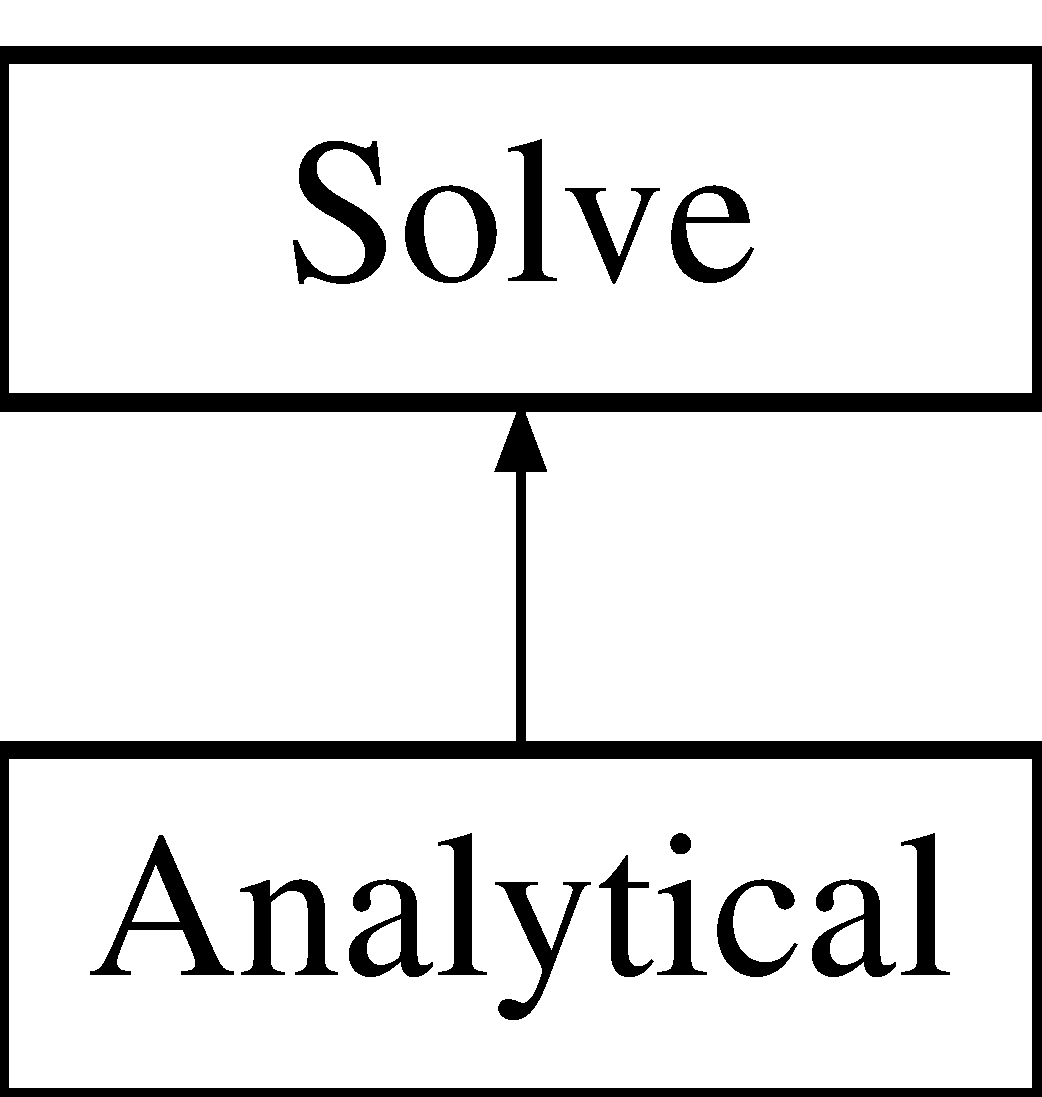
\includegraphics[height=2.000000cm]{class_analytical}
\end{center}
\end{figure}
\subsection*{Public Member Functions}
\begin{DoxyCompactItemize}
\item 
\hyperlink{class_analytical_a5a2be7809dfe198c5d6bdc5b6448f75b}{Analytical} (double D, double Tin, double Tsun, double dt, double dx)
\item 
void \hyperlink{class_analytical_a8fe1d5769bb516115a31719222eb9ae5}{solve} (double t)
\end{DoxyCompactItemize}
\subsection*{Public Attributes}
\begin{DoxyCompactItemize}
\item 
\mbox{\Hypertarget{class_analytical_abee1da12ac56489506088600823328eb}\label{class_analytical_abee1da12ac56489506088600823328eb}} 
\hyperlink{class_vector}{Vector} {\bfseries T}
\item 
\mbox{\Hypertarget{class_analytical_a3a6b8bb5c9985bdfba024ecc378fef14}\label{class_analytical_a3a6b8bb5c9985bdfba024ecc378fef14}} 
int {\bfseries m}
\end{DoxyCompactItemize}


\subsection{Detailed Description}
It\textquotesingle{}s a derived class from \hyperlink{class_solve}{Solve} /n\+It\textquotesingle{}s purpose is to calculate the solution of the problem with the analytical solution ~\newline
-\/T is the solution of the problem ~\newline
-\/m is the number that will remplace infinity in the sum of the analytical solution

The \hyperlink{class_analytical}{Analytical} class provide ~\newline
-\/a basic constructor based on the ine define in the solver class ~\newline
-\/a solve function that will calculate an approximation of T base on the analytical solution, T will be more and more accurate as m grows \begin{DoxySeeAlso}{See also}
\hyperlink{class_solve_a1e0efad6dcf6b09759dd38df7aa08db8}{Solve()} 
\end{DoxySeeAlso}


\subsection{Constructor \& Destructor Documentation}
\mbox{\Hypertarget{class_analytical_a5a2be7809dfe198c5d6bdc5b6448f75b}\label{class_analytical_a5a2be7809dfe198c5d6bdc5b6448f75b}} 
\index{Analytical@{Analytical}!Analytical@{Analytical}}
\index{Analytical@{Analytical}!Analytical@{Analytical}}
\subsubsection{\texorpdfstring{Analytical()}{Analytical()}}
{\footnotesize\ttfamily Analytical\+::\+Analytical (\begin{DoxyParamCaption}\item[{double}]{D,  }\item[{double}]{Tin,  }\item[{double}]{Tsun,  }\item[{double}]{dt,  }\item[{double}]{dx }\end{DoxyParamCaption})}

Default constructor. Based on the \hyperlink{class_solve}{Solve} class constructor, it also define a parameter m and a null vector T

Default constructor -\/  based on the \hyperlink{class_solve}{Solve} class constructor  a value of m high enough for the approximation to be relevant (here 10 000)  the solution vector T as null expect for the two bundary condition 

\subsection{Member Function Documentation}
\mbox{\Hypertarget{class_analytical_a8fe1d5769bb516115a31719222eb9ae5}\label{class_analytical_a8fe1d5769bb516115a31719222eb9ae5}} 
\index{Analytical@{Analytical}!solve@{solve}}
\index{solve@{solve}!Analytical@{Analytical}}
\subsubsection{\texorpdfstring{solve()}{solve()}}
{\footnotesize\ttfamily void Analytical\+::solve (\begin{DoxyParamCaption}\item[{double}]{t }\end{DoxyParamCaption})\hspace{0.3cm}{\ttfamily [virtual]}}

Virtual methods that solve the problem for each scheme depending in which class the objet is define and print it in the consol.  the analytical class it will print the approximate value of T due to the simplicfication of the infinity sum

Virtual method -\/ We use two loop in order to calculate the value of T at each time and each position until the input t is reached. We also print the value of T for every 0.\+1hrs until t is reach 

Reimplemented from \hyperlink{class_solve_a1a56722993fdabea9928637d7dd8a2c7}{Solve}.



The documentation for this class was generated from the following files\+:\begin{DoxyCompactItemize}
\item 
Class/\+Solver/\+Analytical/analytical.\+h\item 
Class/\+Solver/\+Analytical/analytical.\+cpp\end{DoxyCompactItemize}

\hypertarget{class_crank_nicholson}{}\section{Crank\+Nicholson Class Reference}
\label{class_crank_nicholson}\index{Crank\+Nicholson@{Crank\+Nicholson}}


{\ttfamily \#include $<$crank\+Nicholson.\+h$>$}

Inheritance diagram for Crank\+Nicholson\+:\begin{figure}[H]
\begin{center}
\leavevmode
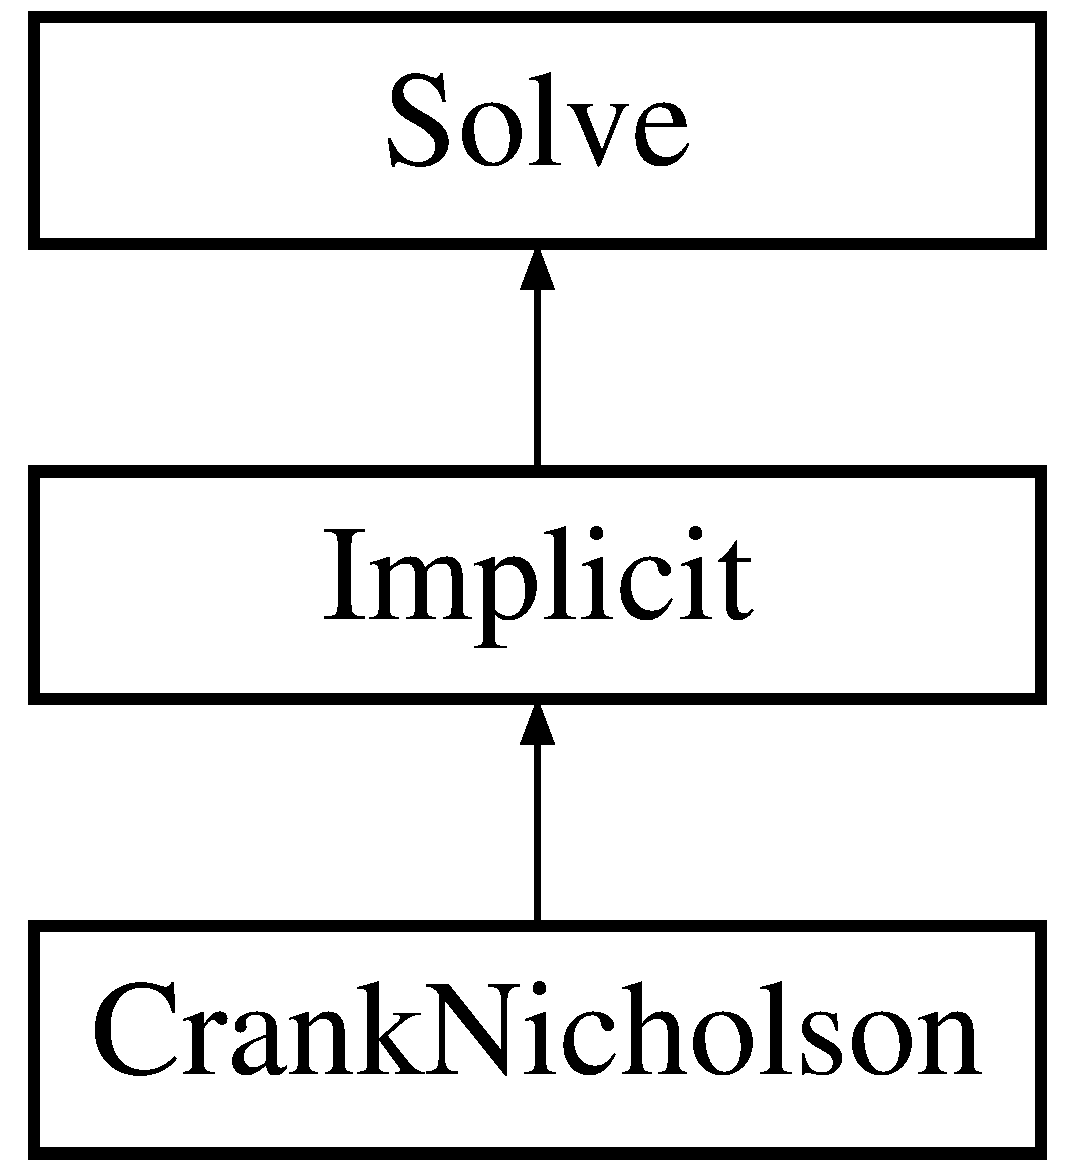
\includegraphics[height=3.000000cm]{class_crank_nicholson}
\end{center}
\end{figure}
\subsection*{Public Member Functions}
\begin{DoxyCompactItemize}
\item 
\hyperlink{class_crank_nicholson_a77c284d244c4c0aabcd2b7d35efc356e}{Crank\+Nicholson} (double \hyperlink{class_solve_ab6b73352e9bca73bad1b133fc84f008c}{D}, double \hyperlink{class_solve_a324c747af91a26a206d7772853b8655e}{Tin}, double \hyperlink{class_solve_a7145536b49fb1ac4d2f36f800d118616}{Tsun}, double \hyperlink{class_solve_ac1befb9c006f895fb0517e19c412ca57}{dt}, double \hyperlink{class_solve_a21b9b8118f508e079f066d2ce2816dd1}{dx})
\item 
void \hyperlink{class_crank_nicholson_a999d04c6ef97b0794f66584f9192dbee}{solve} (double t)
\end{DoxyCompactItemize}
\subsection*{Additional Inherited Members}


\subsection{Detailed Description}
It\textquotesingle{}s a class designed to solved the problem with the Crank-\/\+Nicholson method It\textquotesingle{}s derived from the \hyperlink{class_implicit}{Implicit} class The Crank-\/\+Nicholson class provides\+: ~\newline
-\/basic constructor based on the \hyperlink{class_solve}{Solve} class constructor ~\newline
-\/a virtual solve function that solve the problem with the Crank-\/\+Nicholson scheme 

\subsection{Constructor \& Destructor Documentation}
\mbox{\Hypertarget{class_crank_nicholson_a77c284d244c4c0aabcd2b7d35efc356e}\label{class_crank_nicholson_a77c284d244c4c0aabcd2b7d35efc356e}} 
\index{Crank\+Nicholson@{Crank\+Nicholson}!Crank\+Nicholson@{Crank\+Nicholson}}
\index{Crank\+Nicholson@{Crank\+Nicholson}!Crank\+Nicholson@{Crank\+Nicholson}}
\subsubsection{\texorpdfstring{Crank\+Nicholson()}{CrankNicholson()}}
{\footnotesize\ttfamily Crank\+Nicholson\+::\+Crank\+Nicholson (\begin{DoxyParamCaption}\item[{double}]{D,  }\item[{double}]{Tin,  }\item[{double}]{Tsun,  }\item[{double}]{dt,  }\item[{double}]{dx }\end{DoxyParamCaption})}

Default constructor. Based on the \hyperlink{class_solve}{Solve} constructor and implicit constuctor \begin{DoxySeeAlso}{See also}
\hyperlink{class_solve_a1e0efad6dcf6b09759dd38df7aa08db8}{Solve(double D, double Tin, double Tsun, double dt, double dx)} 

\hyperlink{class_implicit_afe5ef51232ab8925009f584c679bdfce}{Implicit(double D, double Tin, double Tsun, double dt, double dx)}
\end{DoxySeeAlso}
Default constructor -\/ Based on the Solver and \hyperlink{class_implicit}{Implicit} constructor We implement the value of a and b use in the \hyperlink{class_implicit}{Implicit} class \begin{DoxySeeAlso}{See also}
\hyperlink{class_implicit_a572fff2232977c83c432f993f37a7853}{Diagonalization(\+Vector \&\+T)} 
\end{DoxySeeAlso}


\subsection{Member Function Documentation}
\mbox{\Hypertarget{class_crank_nicholson_a999d04c6ef97b0794f66584f9192dbee}\label{class_crank_nicholson_a999d04c6ef97b0794f66584f9192dbee}} 
\index{Crank\+Nicholson@{Crank\+Nicholson}!solve@{solve}}
\index{solve@{solve}!Crank\+Nicholson@{Crank\+Nicholson}}
\subsubsection{\texorpdfstring{solve()}{solve()}}
{\footnotesize\ttfamily void Crank\+Nicholson\+::solve (\begin{DoxyParamCaption}\item[{double}]{t }\end{DoxyParamCaption})\hspace{0.3cm}{\ttfamily [virtual]}}

Virtual methods that solve the problem for each scheme depending in which class the objet is define and print the result in the consol. ~\newline
 \hyperlink{class_solve}{Solve} the problem using the Crank-\/\+Nicholson scheme \begin{DoxySeeAlso}{See also}
\hyperlink{class_implicit_a572fff2232977c83c432f993f37a7853}{Diagonalization(\+Vector \&\+T)}
\end{DoxySeeAlso}
Virtual method -\/ \hyperlink{class_solve}{Solve} the problem with the Cranck-\/\+Nicholson scheme 

Reimplemented from \hyperlink{class_solve_a1a56722993fdabea9928637d7dd8a2c7}{Solve}.



The documentation for this class was generated from the following files\+:\begin{DoxyCompactItemize}
\item 
Solver/\+Implicit/\+Crank-\/\+Nicholson/\hyperlink{crank_nicholson_8h}{crank\+Nicholson.\+h}\item 
Solver/\+Implicit/\+Crank-\/\+Nicholson/\hyperlink{crank_nicholson_8cpp}{crank\+Nicholson.\+cpp}\end{DoxyCompactItemize}

\hypertarget{class_du_fort_frankel}{}\section{Du\+Fort\+Frankel Class Reference}
\label{class_du_fort_frankel}\index{Du\+Fort\+Frankel@{Du\+Fort\+Frankel}}


{\ttfamily \#include $<$du\+Fort\+Frankel.\+h$>$}

Inheritance diagram for Du\+Fort\+Frankel\+:\begin{figure}[H]
\begin{center}
\leavevmode
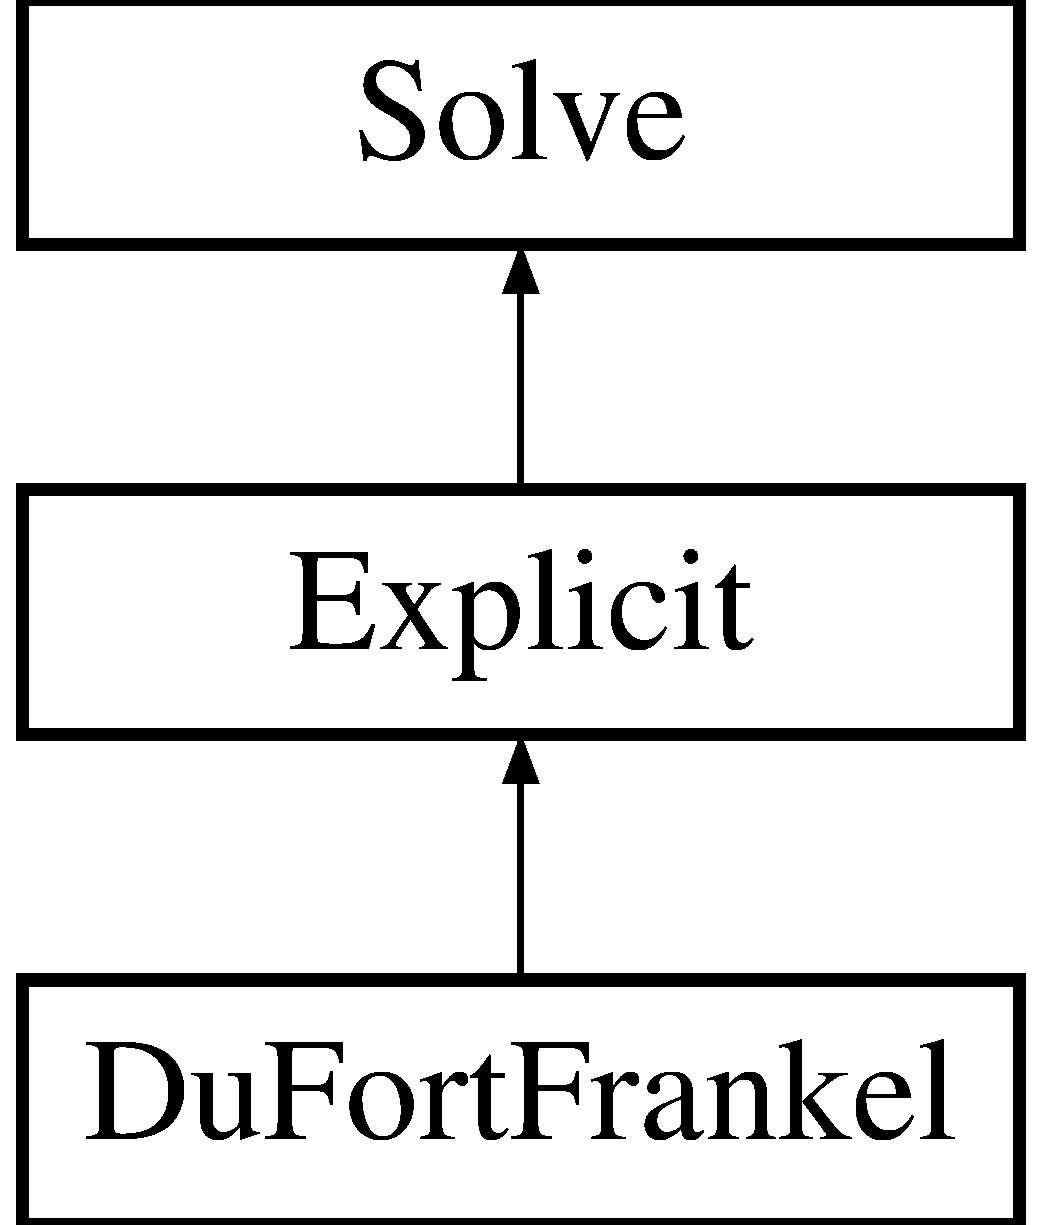
\includegraphics[height=3.000000cm]{class_du_fort_frankel}
\end{center}
\end{figure}
\subsection*{Public Member Functions}
\begin{DoxyCompactItemize}
\item 
\hyperlink{class_du_fort_frankel_ab9a6490d0fd3b08e7e22fba2ade16c19}{Du\+Fort\+Frankel} (double \hyperlink{class_solve_ab6b73352e9bca73bad1b133fc84f008c}{D}, double \hyperlink{class_solve_a324c747af91a26a206d7772853b8655e}{Tin}, double \hyperlink{class_solve_a7145536b49fb1ac4d2f36f800d118616}{Tsun}, double \hyperlink{class_solve_ac1befb9c006f895fb0517e19c412ca57}{dt}, double \hyperlink{class_solve_a21b9b8118f508e079f066d2ce2816dd1}{dx})
\item 
void \hyperlink{class_du_fort_frankel_a73204223c7ace1e3f95e5d89d02c5208}{solve} (double t)
\end{DoxyCompactItemize}
\subsection*{Additional Inherited Members}


\subsection{Detailed Description}
It\textquotesingle{}s a class designed to solved the problem with the Du\+Fort-\/\+Frankel method It\textquotesingle{}s derived from the \hyperlink{class_explicit}{Explicit} class

The \hyperlink{class_du_fort_frankel}{Du\+Fort\+Frankel} class provides\+: ~\newline
-\/basic constructor based on the \hyperlink{class_solve}{Solve} class constructor ~\newline
-\/a virtual solve function that solve the problem with the Du\+Fort-\/\+Frankel scheme 

\subsection{Constructor \& Destructor Documentation}
\mbox{\Hypertarget{class_du_fort_frankel_ab9a6490d0fd3b08e7e22fba2ade16c19}\label{class_du_fort_frankel_ab9a6490d0fd3b08e7e22fba2ade16c19}} 
\index{Du\+Fort\+Frankel@{Du\+Fort\+Frankel}!Du\+Fort\+Frankel@{Du\+Fort\+Frankel}}
\index{Du\+Fort\+Frankel@{Du\+Fort\+Frankel}!Du\+Fort\+Frankel@{Du\+Fort\+Frankel}}
\subsubsection{\texorpdfstring{Du\+Fort\+Frankel()}{DuFortFrankel()}}
{\footnotesize\ttfamily Du\+Fort\+Frankel\+::\+Du\+Fort\+Frankel (\begin{DoxyParamCaption}\item[{double}]{D,  }\item[{double}]{Tin,  }\item[{double}]{Tsun,  }\item[{double}]{dt,  }\item[{double}]{dx }\end{DoxyParamCaption})}

Default constructor. Based on the \hyperlink{class_solve}{Solve} constructor \begin{DoxySeeAlso}{See also}
\hyperlink{class_solve_a1e0efad6dcf6b09759dd38df7aa08db8}{Solve(double D, double Tin, double Tsun, double dt, double dx)} 

\hyperlink{class_explicit_ab5b890fae2ea8a91c95e9a15f552f36a}{Explicit(double D, double Tin, double Tsun, double dt, double dx)}
\end{DoxySeeAlso}
Default constructor -\/ Based on the Solver constructor 

\subsection{Member Function Documentation}
\mbox{\Hypertarget{class_du_fort_frankel_a73204223c7ace1e3f95e5d89d02c5208}\label{class_du_fort_frankel_a73204223c7ace1e3f95e5d89d02c5208}} 
\index{Du\+Fort\+Frankel@{Du\+Fort\+Frankel}!solve@{solve}}
\index{solve@{solve}!Du\+Fort\+Frankel@{Du\+Fort\+Frankel}}
\subsubsection{\texorpdfstring{solve()}{solve()}}
{\footnotesize\ttfamily void Du\+Fort\+Frankel\+::solve (\begin{DoxyParamCaption}\item[{double}]{t }\end{DoxyParamCaption})\hspace{0.3cm}{\ttfamily [virtual]}}

Virtual methods that solve the problem for each scheme depending in which class the objet is define and print the result in the consol. ~\newline
 \hyperlink{class_solve}{Solve} the problem using the \hyperlink{class_du_fort_frankel}{Du\+Fort\+Frankel} scheme \begin{DoxySeeAlso}{See also}
\hyperlink{class_explicit_a6069720017eb2bb0d989b2557c162c97}{Order\+One(\+Vector \&\+T)}
\end{DoxySeeAlso}
Virtual method -\/ \hyperlink{class_solve}{Solve} the problem with the Du\+Fort-\/\+Frankel scheme 

Reimplemented from \hyperlink{class_solve_a1a56722993fdabea9928637d7dd8a2c7}{Solve}.



The documentation for this class was generated from the following files\+:\begin{DoxyCompactItemize}
\item 
Solver/\+Explicit/\+Du\+Fort-\/\+Frankel/\hyperlink{du_fort_frankel_8h}{du\+Fort\+Frankel.\+h}\item 
Solver/\+Explicit/\+Du\+Fort-\/\+Frankel/\hyperlink{du_fort_frankel_8cpp}{du\+Fort\+Frankel.\+cpp}\end{DoxyCompactItemize}

\hypertarget{class_explicit}{}\section{Explicit Class Reference}
\label{class_explicit}\index{Explicit@{Explicit}}


{\ttfamily \#include $<$explicit.\+h$>$}

Inheritance diagram for Explicit\+:\begin{figure}[H]
\begin{center}
\leavevmode
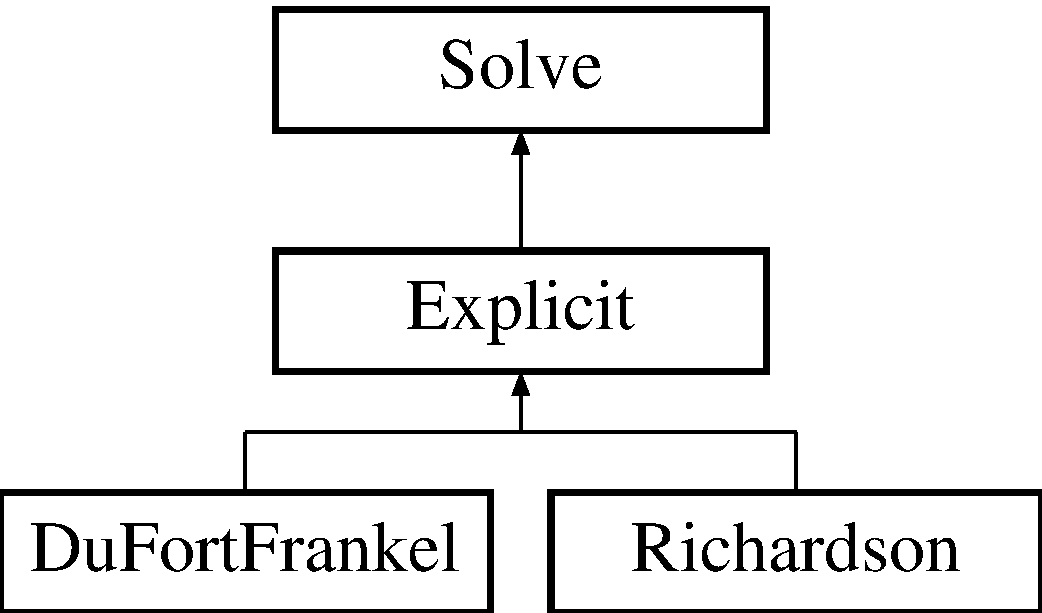
\includegraphics[height=3.000000cm]{class_explicit}
\end{center}
\end{figure}
\subsection*{Public Member Functions}
\begin{DoxyCompactItemize}
\item 
\hyperlink{class_explicit_ab5b890fae2ea8a91c95e9a15f552f36a}{Explicit} (double D, double Tin, double Tsun, double dt, double dx)
\item 
void \hyperlink{class_explicit_ac99aa17bfd95f66b33e5c0ecf0e53785}{solve} (double t)
\item 
void \hyperlink{class_explicit_a6069720017eb2bb0d989b2557c162c97}{Order\+One} (\hyperlink{class_vector}{Vector} \&T)
\end{DoxyCompactItemize}
\subsection*{Additional Inherited Members}


\subsection{Detailed Description}
This class is derived from the \hyperlink{class_solve}{Solve} class and is the base class of the two explicit scheme Class, \hyperlink{class_du_fort_frankel}{Du\+Fort\+Frankel} and \hyperlink{class_richardson}{Richardson}.

The \hyperlink{class_explicit}{Explicit} class provides\+: ~\newline
-\/basic constructor derived from \hyperlink{class_solve}{Solve} ~\newline
-\/a virtual function \hyperlink{class_explicit_ac99aa17bfd95f66b33e5c0ecf0e53785}{solve()} that will be use in the derived function to solve the problem ~\newline
-\/a \begin{DoxySeeAlso}{See also}
Ordern\+One(\+Vector \&\+T) function that will be used in both derived class to calculate the first term needed to apply the schemes 
\end{DoxySeeAlso}


\subsection{Constructor \& Destructor Documentation}
\mbox{\Hypertarget{class_explicit_ab5b890fae2ea8a91c95e9a15f552f36a}\label{class_explicit_ab5b890fae2ea8a91c95e9a15f552f36a}} 
\index{Explicit@{Explicit}!Explicit@{Explicit}}
\index{Explicit@{Explicit}!Explicit@{Explicit}}
\subsubsection{\texorpdfstring{Explicit()}{Explicit()}}
{\footnotesize\ttfamily Explicit\+::\+Explicit (\begin{DoxyParamCaption}\item[{double}]{D,  }\item[{double}]{Tin,  }\item[{double}]{Tsun,  }\item[{double}]{dt,  }\item[{double}]{dx }\end{DoxyParamCaption})}

Default constructor. Based on the \hyperlink{class_solve}{Solve} constructor \begin{DoxySeeAlso}{See also}
\hyperlink{class_solve_a1e0efad6dcf6b09759dd38df7aa08db8}{Solve()}
\end{DoxySeeAlso}
Default constructor -\/ Same as the Soler constructor 

\subsection{Member Function Documentation}
\mbox{\Hypertarget{class_explicit_a6069720017eb2bb0d989b2557c162c97}\label{class_explicit_a6069720017eb2bb0d989b2557c162c97}} 
\index{Explicit@{Explicit}!Order\+One@{Order\+One}}
\index{Order\+One@{Order\+One}!Explicit@{Explicit}}
\subsubsection{\texorpdfstring{Order\+One()}{OrderOne()}}
{\footnotesize\ttfamily void Explicit\+::\+Order\+One (\begin{DoxyParamCaption}\item[{\hyperlink{class_vector}{Vector} \&}]{T }\end{DoxyParamCaption})}

Void method that will change the value of the \hyperlink{class_vector}{Vector} T and calculate the first scheme with a forward time central space scheme

Void methods that initialize T at t=0 and calculate T at t = dt \mbox{\Hypertarget{class_explicit_ac99aa17bfd95f66b33e5c0ecf0e53785}\label{class_explicit_ac99aa17bfd95f66b33e5c0ecf0e53785}} 
\index{Explicit@{Explicit}!solve@{solve}}
\index{solve@{solve}!Explicit@{Explicit}}
\subsubsection{\texorpdfstring{solve()}{solve()}}
{\footnotesize\ttfamily void Explicit\+::solve (\begin{DoxyParamCaption}\item[{double}]{t }\end{DoxyParamCaption})\hspace{0.3cm}{\ttfamily [virtual]}}

Virtual methods that solve the problem for each scheme depending in which class the objet is define and print it in the consol.  the \hyperlink{class_explicit}{Explicit} class it doesn\textquotesingle{}t do anything

Virtual method -\/ Not defined here 

Reimplemented from \hyperlink{class_solve_a1a56722993fdabea9928637d7dd8a2c7}{Solve}.



Reimplemented in \hyperlink{class_richardson_ab8dd2ff0e58c11092fead4d45a4f5c64}{Richardson}.



The documentation for this class was generated from the following files\+:\begin{DoxyCompactItemize}
\item 
Class/\+Solver/\+Explicit/explicit.\+h\item 
Class/\+Solver/\+Explicit/explicit.\+cpp\end{DoxyCompactItemize}

\hypertarget{class_implicit}{}\section{Implicit Class Reference}
\label{class_implicit}\index{Implicit@{Implicit}}


{\ttfamily \#include $<$implicit.\+h$>$}

Inheritance diagram for Implicit\+:\begin{figure}[H]
\begin{center}
\leavevmode
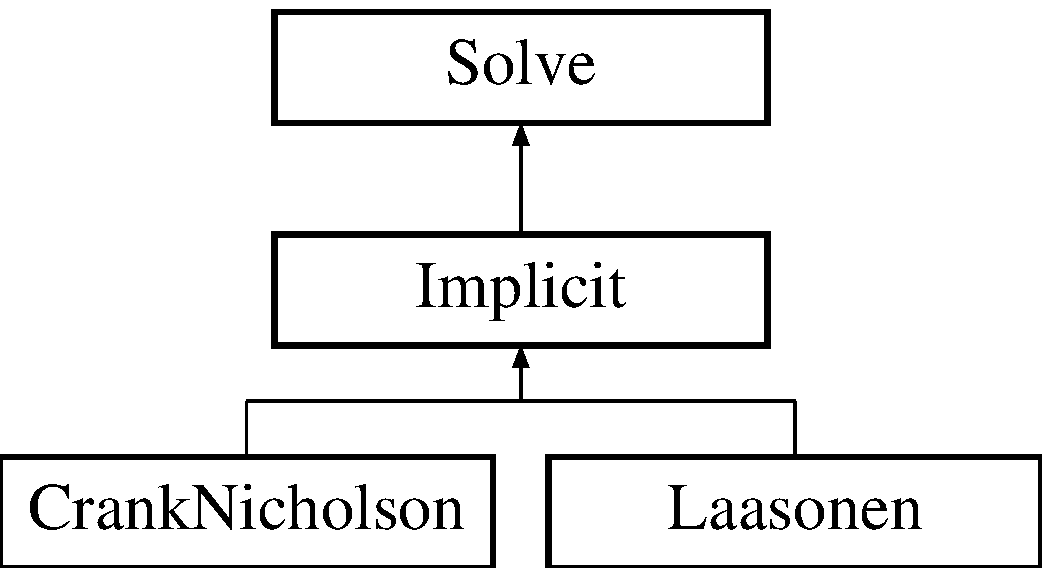
\includegraphics[height=3.000000cm]{class_implicit}
\end{center}
\end{figure}
\subsection*{Public Member Functions}
\begin{DoxyCompactItemize}
\item 
\hyperlink{class_implicit_a5a98f30bdf419368901ce9468a7065a3}{Implicit} ()
\item 
\hyperlink{class_implicit_afe5ef51232ab8925009f584c679bdfce}{Implicit} (double \hyperlink{class_solve_ab6b73352e9bca73bad1b133fc84f008c}{D}, double \hyperlink{class_solve_a324c747af91a26a206d7772853b8655e}{Tin}, double \hyperlink{class_solve_a7145536b49fb1ac4d2f36f800d118616}{Tsun}, double \hyperlink{class_solve_ac1befb9c006f895fb0517e19c412ca57}{dt}, double \hyperlink{class_solve_a21b9b8118f508e079f066d2ce2816dd1}{dx})
\item 
void \hyperlink{class_implicit_a027adb4276376991f75fcffbd34740b3}{solve} (double t)
\item 
void \hyperlink{class_implicit_a572fff2232977c83c432f993f37a7853}{Diagonalization} (\hyperlink{class_vector}{Vector} \&T)
\end{DoxyCompactItemize}
\subsection*{Public Attributes}
\begin{DoxyCompactItemize}
\item 
double \hyperlink{class_implicit_a58a95622ffc58ae2f468d3ef4f0d215c}{a}
\item 
double \hyperlink{class_implicit_a270615b52e1106f89b4e6ef928cc12de}{b}
\item 
\hyperlink{class_vector}{Vector} \hyperlink{class_implicit_a5bdc685b164fc363d26ed1461c0d49b2}{A}
\item 
\hyperlink{class_vector}{Vector} \hyperlink{class_implicit_a3f9c9eda634c19c2301698fd81ec5a6b}{B}
\item 
\hyperlink{class_vector}{Vector} \hyperlink{class_implicit_a854215cf2128a1dc1f532bb6664b472c}{Tnext}
\item 
\hyperlink{class_vector}{Vector} \hyperlink{class_implicit_a6cd9e0093600402e8bc3b22995aa96b1}{Tpast}
\end{DoxyCompactItemize}


\subsection{Detailed Description}
This class is derived from the \hyperlink{class_solve}{Solve} class and is the base class of the two implicit scheme Class, Crank-\/\+Nicholson and \hyperlink{class_laasonen}{Laasonen}.

The \hyperlink{class_implicit}{Implicit} class provides\+: ~\newline
-\/basic constructor derived from \hyperlink{class_solve}{Solve} ~\newline
-\/a virtual function \hyperlink{class_implicit_a027adb4276376991f75fcffbd34740b3}{solve()} that will be use in the derived function to solve the problem ~\newline
-\/a \begin{DoxySeeAlso}{See also}
\hyperlink{class_implicit_a572fff2232977c83c432f993f37a7853}{Diagonalization(\+Vector \&\+T)} function that will be used in both derived class to calculate the first part of the thomas Algorithm (\hyperlink{class_implicit_a572fff2232977c83c432f993f37a7853}{Diagonalization} and resolving the equation Ly = \hyperlink{class_implicit_a270615b52e1106f89b4e6ef928cc12de}{b} ) 
\end{DoxySeeAlso}


\subsection{Constructor \& Destructor Documentation}
\mbox{\Hypertarget{class_implicit_a5a98f30bdf419368901ce9468a7065a3}\label{class_implicit_a5a98f30bdf419368901ce9468a7065a3}} 
\index{Implicit@{Implicit}!Implicit@{Implicit}}
\index{Implicit@{Implicit}!Implicit@{Implicit}}
\subsubsection{\texorpdfstring{Implicit()}{Implicit()}\hspace{0.1cm}{\footnotesize\ttfamily [1/2]}}
{\footnotesize\ttfamily Implicit\+::\+Implicit (\begin{DoxyParamCaption}{ }\end{DoxyParamCaption})}

Default constructor. Set all the value expect n to 0 \begin{DoxySeeAlso}{See also}
\hyperlink{class_solve_ac437f1307c9d4669205ac7d370a55ffc}{Solve()} 

\hyperlink{class_implicit_afe5ef51232ab8925009f584c679bdfce}{Implicit(double D, double Tin, double Tsun, double dt, double dx)}
\end{DoxySeeAlso}
Default constructor -\/ Same as the Solver constructor set all the value to one \mbox{\Hypertarget{class_implicit_afe5ef51232ab8925009f584c679bdfce}\label{class_implicit_afe5ef51232ab8925009f584c679bdfce}} 
\index{Implicit@{Implicit}!Implicit@{Implicit}}
\index{Implicit@{Implicit}!Implicit@{Implicit}}
\subsubsection{\texorpdfstring{Implicit()}{Implicit()}\hspace{0.1cm}{\footnotesize\ttfamily [2/2]}}
{\footnotesize\ttfamily Implicit\+::\+Implicit (\begin{DoxyParamCaption}\item[{double}]{D,  }\item[{double}]{Tin,  }\item[{double}]{Tsun,  }\item[{double}]{dt,  }\item[{double}]{dx }\end{DoxyParamCaption})}

Based on the \hyperlink{class_solve}{Solve} constructor \begin{DoxySeeAlso}{See also}
\hyperlink{class_solve_a1e0efad6dcf6b09759dd38df7aa08db8}{Solve(double D, double Tin, double Tsun, double dt, double dx)}
\end{DoxySeeAlso}
Constructor -\/ Same as the Soler constructor, we initialise the two vectors A and B 

\subsection{Member Function Documentation}
\mbox{\Hypertarget{class_implicit_a572fff2232977c83c432f993f37a7853}\label{class_implicit_a572fff2232977c83c432f993f37a7853}} 
\index{Implicit@{Implicit}!Diagonalization@{Diagonalization}}
\index{Diagonalization@{Diagonalization}!Implicit@{Implicit}}
\subsubsection{\texorpdfstring{Diagonalization()}{Diagonalization()}}
{\footnotesize\ttfamily void Implicit\+::\+Diagonalization (\begin{DoxyParamCaption}\item[{\hyperlink{class_vector}{Vector} \&}]{T }\end{DoxyParamCaption})}

Void method that will change that will use the \hyperlink{class_vector}{Vector} T and calculate the first part of the thomas alrgorithm by changing the value of the vectors A and B that will be use in the derived class solve function

It has no interset to use this function in the \hyperlink{class_implicit}{Implicit} class cause it uses parameters defined in the derived classes (a and b)

Void methods that implement the first part of the thomas algorithm \mbox{\Hypertarget{class_implicit_a027adb4276376991f75fcffbd34740b3}\label{class_implicit_a027adb4276376991f75fcffbd34740b3}} 
\index{Implicit@{Implicit}!solve@{solve}}
\index{solve@{solve}!Implicit@{Implicit}}
\subsubsection{\texorpdfstring{solve()}{solve()}}
{\footnotesize\ttfamily void Implicit\+::solve (\begin{DoxyParamCaption}\item[{double}]{t }\end{DoxyParamCaption})\hspace{0.3cm}{\ttfamily [virtual]}}

Virtual methods that solve the problem for each scheme depending in which class the objet is define and print it in the consol.  the \hyperlink{class_implicit}{Implicit} class it doesn\textquotesingle{}t do anything

Virtual method -\/ Not defined here 

Reimplemented from \hyperlink{class_solve_a1a56722993fdabea9928637d7dd8a2c7}{Solve}.



Reimplemented in \hyperlink{class_laasonen_aaa49ab7d15fbfef94a57a0e89977d1c6}{Laasonen}.



\subsection{Member Data Documentation}
\mbox{\Hypertarget{class_implicit_a58a95622ffc58ae2f468d3ef4f0d215c}\label{class_implicit_a58a95622ffc58ae2f468d3ef4f0d215c}} 
\index{Implicit@{Implicit}!a@{a}}
\index{a@{a}!Implicit@{Implicit}}
\subsubsection{\texorpdfstring{a}{a}}
{\footnotesize\ttfamily double Implicit\+::a}

\mbox{\Hypertarget{class_implicit_a5bdc685b164fc363d26ed1461c0d49b2}\label{class_implicit_a5bdc685b164fc363d26ed1461c0d49b2}} 
\index{Implicit@{Implicit}!A@{A}}
\index{A@{A}!Implicit@{Implicit}}
\subsubsection{\texorpdfstring{A}{A}}
{\footnotesize\ttfamily \hyperlink{class_vector}{Vector} Implicit\+::A}

\mbox{\Hypertarget{class_implicit_a270615b52e1106f89b4e6ef928cc12de}\label{class_implicit_a270615b52e1106f89b4e6ef928cc12de}} 
\index{Implicit@{Implicit}!b@{b}}
\index{b@{b}!Implicit@{Implicit}}
\subsubsection{\texorpdfstring{b}{b}}
{\footnotesize\ttfamily double Implicit\+::b}

\mbox{\Hypertarget{class_implicit_a3f9c9eda634c19c2301698fd81ec5a6b}\label{class_implicit_a3f9c9eda634c19c2301698fd81ec5a6b}} 
\index{Implicit@{Implicit}!B@{B}}
\index{B@{B}!Implicit@{Implicit}}
\subsubsection{\texorpdfstring{B}{B}}
{\footnotesize\ttfamily \hyperlink{class_vector}{Vector} Implicit\+::B}

\mbox{\Hypertarget{class_implicit_a854215cf2128a1dc1f532bb6664b472c}\label{class_implicit_a854215cf2128a1dc1f532bb6664b472c}} 
\index{Implicit@{Implicit}!Tnext@{Tnext}}
\index{Tnext@{Tnext}!Implicit@{Implicit}}
\subsubsection{\texorpdfstring{Tnext}{Tnext}}
{\footnotesize\ttfamily \hyperlink{class_vector}{Vector} Implicit\+::\+Tnext}

\mbox{\Hypertarget{class_implicit_a6cd9e0093600402e8bc3b22995aa96b1}\label{class_implicit_a6cd9e0093600402e8bc3b22995aa96b1}} 
\index{Implicit@{Implicit}!Tpast@{Tpast}}
\index{Tpast@{Tpast}!Implicit@{Implicit}}
\subsubsection{\texorpdfstring{Tpast}{Tpast}}
{\footnotesize\ttfamily \hyperlink{class_vector}{Vector} Implicit\+::\+Tpast}



The documentation for this class was generated from the following files\+:\begin{DoxyCompactItemize}
\item 
Solver/\+Implicit/\hyperlink{implicit_8h}{implicit.\+h}\item 
Solver/\+Implicit/\hyperlink{implicit_8cpp}{implicit.\+cpp}\end{DoxyCompactItemize}

\hypertarget{class_laasonen}{}\section{Laasonen Class Reference}
\label{class_laasonen}\index{Laasonen@{Laasonen}}


{\ttfamily \#include $<$laasonen.\+h$>$}

Inheritance diagram for Laasonen\+:\begin{figure}[H]
\begin{center}
\leavevmode
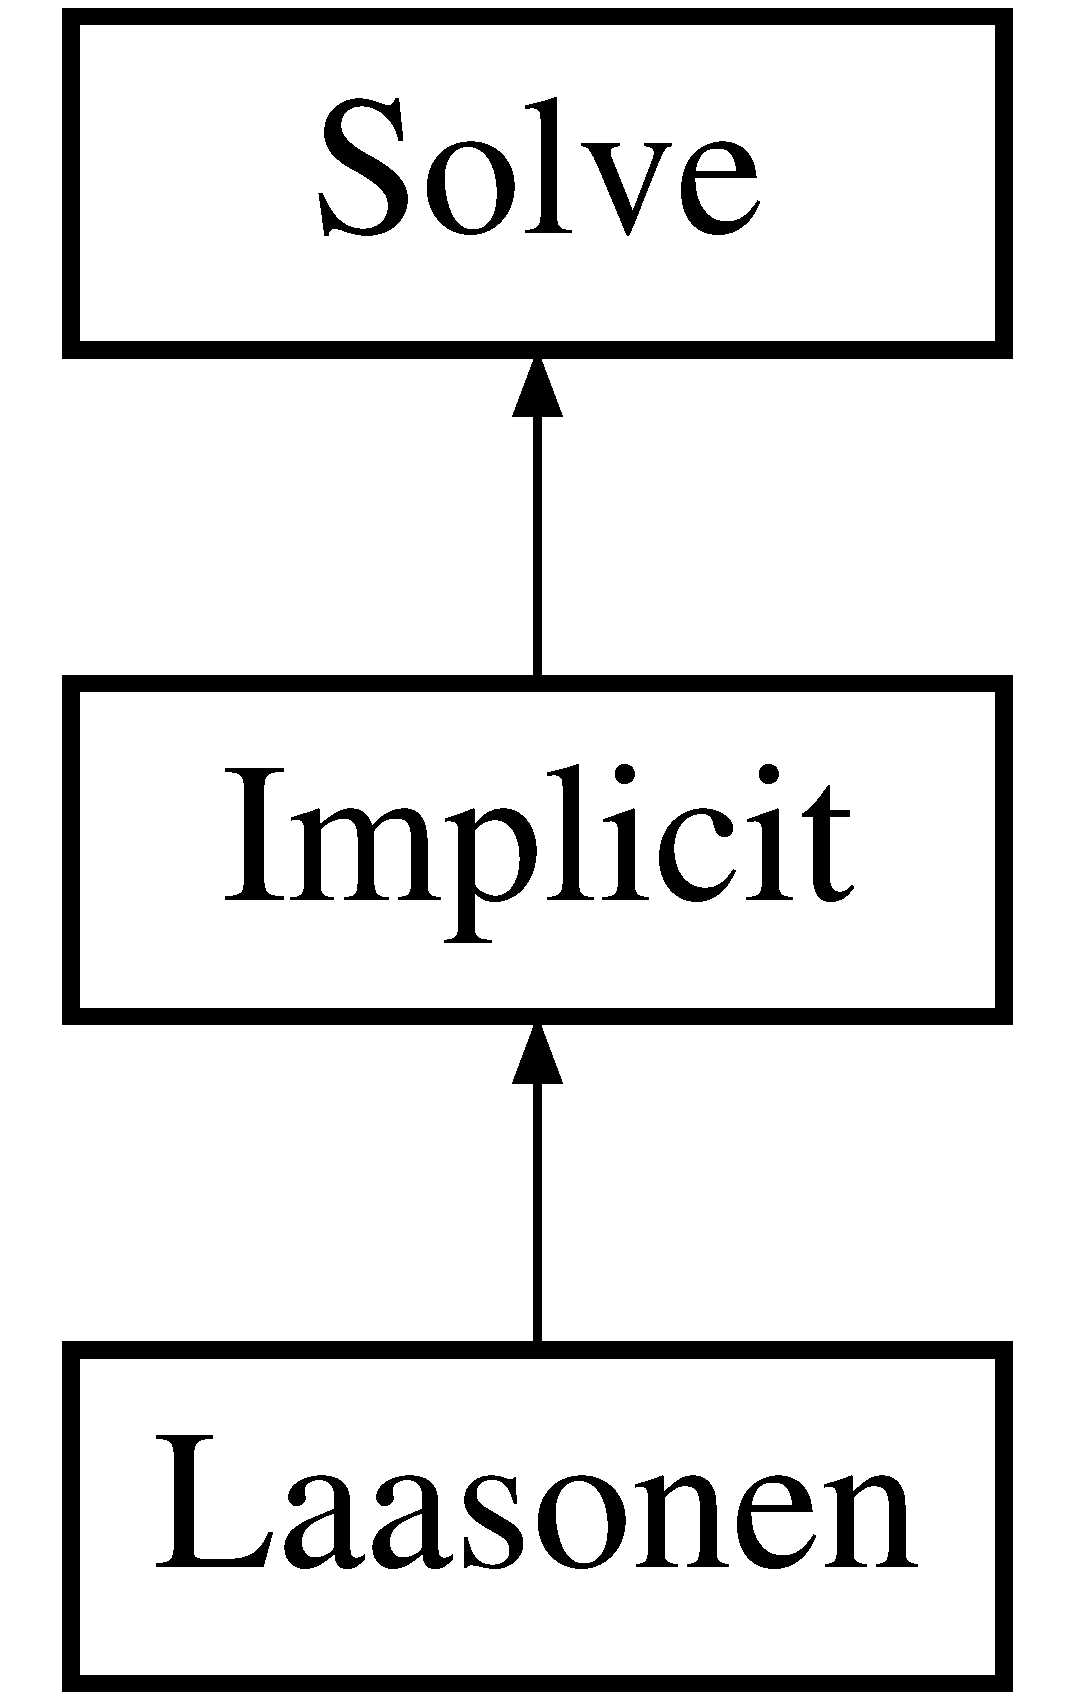
\includegraphics[height=3.000000cm]{class_laasonen}
\end{center}
\end{figure}
\subsection*{Public Member Functions}
\begin{DoxyCompactItemize}
\item 
\hyperlink{class_laasonen_ad20d5e371558ef7c4f04f730daef0049}{Laasonen} (double \hyperlink{class_solve_ab6b73352e9bca73bad1b133fc84f008c}{D}, double \hyperlink{class_solve_a324c747af91a26a206d7772853b8655e}{Tin}, double \hyperlink{class_solve_a7145536b49fb1ac4d2f36f800d118616}{Tsun}, double \hyperlink{class_solve_ac1befb9c006f895fb0517e19c412ca57}{dt}, double \hyperlink{class_solve_a21b9b8118f508e079f066d2ce2816dd1}{dx})
\item 
void \hyperlink{class_laasonen_aaa49ab7d15fbfef94a57a0e89977d1c6}{solve} (double t)
\end{DoxyCompactItemize}
\subsection*{Additional Inherited Members}


\subsection{Detailed Description}
It\textquotesingle{}s a class designed to solved the problem with the \hyperlink{class_laasonen}{Laasonen} method It\textquotesingle{}s derived from the \hyperlink{class_implicit}{Implicit} class The \hyperlink{class_laasonen}{Laasonen} class provides\+: ~\newline
-\/basic constructor based on the \hyperlink{class_solve}{Solve} class constructor ~\newline
-\/a virtual solve function that solve the problem with the \hyperlink{class_laasonen}{Laasonen} scheme 

\subsection{Constructor \& Destructor Documentation}
\mbox{\Hypertarget{class_laasonen_ad20d5e371558ef7c4f04f730daef0049}\label{class_laasonen_ad20d5e371558ef7c4f04f730daef0049}} 
\index{Laasonen@{Laasonen}!Laasonen@{Laasonen}}
\index{Laasonen@{Laasonen}!Laasonen@{Laasonen}}
\subsubsection{\texorpdfstring{Laasonen()}{Laasonen()}}
{\footnotesize\ttfamily Laasonen\+::\+Laasonen (\begin{DoxyParamCaption}\item[{double}]{D,  }\item[{double}]{Tin,  }\item[{double}]{Tsun,  }\item[{double}]{dt,  }\item[{double}]{dx }\end{DoxyParamCaption})}

Default constructor. Based on the \hyperlink{class_solve}{Solve} constructor and implicit constuctor \begin{DoxySeeAlso}{See also}
\hyperlink{class_solve_a1e0efad6dcf6b09759dd38df7aa08db8}{Solve(double D, double Tin, double Tsun, double dt, double dx)} 

\hyperlink{class_implicit_afe5ef51232ab8925009f584c679bdfce}{Implicit(double D, double Tin, double Tsun, double dt, double dx)}
\end{DoxySeeAlso}
Default constructor -\/ Based on the Solver and \hyperlink{class_implicit}{Implicit} constructor We implement the value of a and b use in the \hyperlink{class_implicit}{Implicit} class \begin{DoxySeeAlso}{See also}
\hyperlink{class_implicit_a572fff2232977c83c432f993f37a7853}{Diagonalization(\+Vector \&\+T)} 
\end{DoxySeeAlso}


\subsection{Member Function Documentation}
\mbox{\Hypertarget{class_laasonen_aaa49ab7d15fbfef94a57a0e89977d1c6}\label{class_laasonen_aaa49ab7d15fbfef94a57a0e89977d1c6}} 
\index{Laasonen@{Laasonen}!solve@{solve}}
\index{solve@{solve}!Laasonen@{Laasonen}}
\subsubsection{\texorpdfstring{solve()}{solve()}}
{\footnotesize\ttfamily void Laasonen\+::solve (\begin{DoxyParamCaption}\item[{double}]{t }\end{DoxyParamCaption})\hspace{0.3cm}{\ttfamily [virtual]}}

Virtual methods that solve the problem for each scheme depending in which class the objet is define and print the result in the consol. ~\newline
 \hyperlink{class_solve}{Solve} the problem using the \hyperlink{class_laasonen}{Laasonen} scheme \begin{DoxySeeAlso}{See also}
\hyperlink{class_implicit_a572fff2232977c83c432f993f37a7853}{Diagonalization(\+Vector \&\+T)}
\end{DoxySeeAlso}
Virtual method -\/ \hyperlink{class_solve}{Solve} the problem with the \hyperlink{class_laasonen}{Laasonen} scheme 

Reimplemented from \hyperlink{class_implicit_a027adb4276376991f75fcffbd34740b3}{Implicit}.



The documentation for this class was generated from the following files\+:\begin{DoxyCompactItemize}
\item 
Solver/\+Implicit/\+Laasonen/\hyperlink{laasonen_8h}{laasonen.\+h}\item 
Solver/\+Implicit/\+Laasonen/\hyperlink{laasonen_8cpp}{laasonen.\+cpp}\end{DoxyCompactItemize}

\hypertarget{class_richardson}{}\section{Richardson Class Reference}
\label{class_richardson}\index{Richardson@{Richardson}}


{\ttfamily \#include $<$richardson.\+h$>$}

Inheritance diagram for Richardson\+:\begin{figure}[H]
\begin{center}
\leavevmode
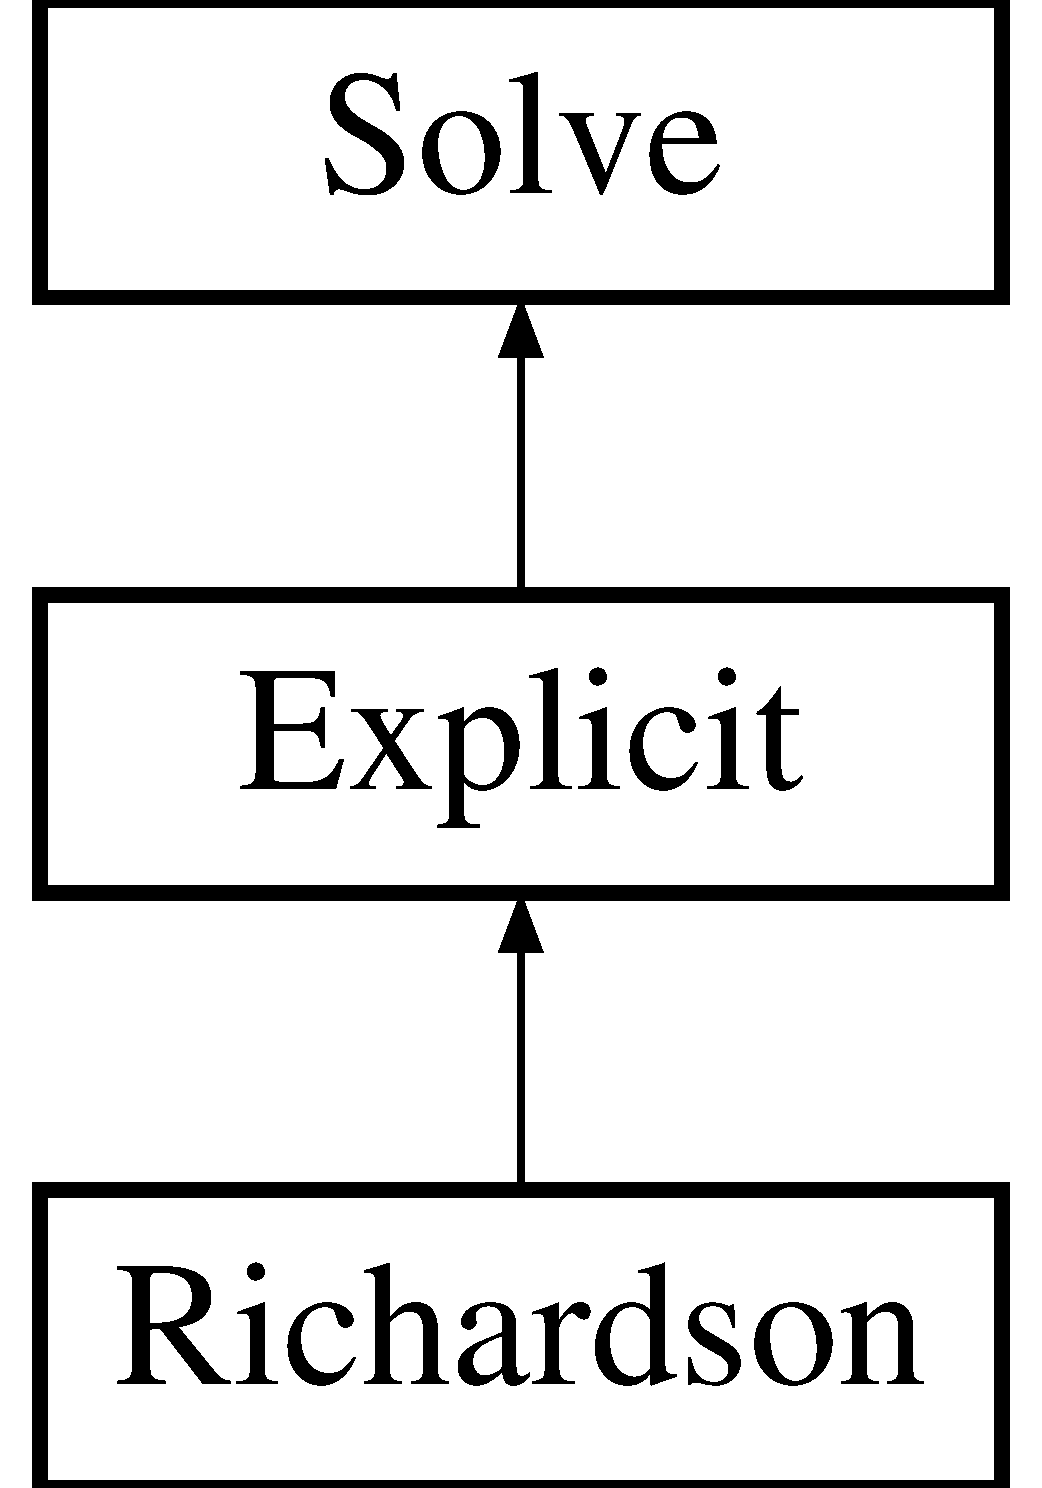
\includegraphics[height=3.000000cm]{class_richardson}
\end{center}
\end{figure}
\subsection*{Public Member Functions}
\begin{DoxyCompactItemize}
\item 
\hyperlink{class_richardson_ab669d2d69be9d899d5ca2bb7a7c33a5b}{Richardson} (double D, double Tin, double Tsun, double dt, double dx)
\item 
void \hyperlink{class_richardson_ab8dd2ff0e58c11092fead4d45a4f5c64}{solve} (double t)
\end{DoxyCompactItemize}
\subsection*{Additional Inherited Members}


\subsection{Detailed Description}
It\textquotesingle{}s a class designed to solved the problem with the \hyperlink{class_richardson}{Richardson} method It\textquotesingle{}s derived from the \hyperlink{class_explicit}{Explicit} class

The \hyperlink{class_richardson}{Richardson} class provides\+: ~\newline
-\/basic constructor based on the \hyperlink{class_solve}{Solve} class constructor ~\newline
-\/a virtual solve function that solve the problem with the \hyperlink{class_richardson}{Richardson} scheme 

\subsection{Constructor \& Destructor Documentation}
\mbox{\Hypertarget{class_richardson_ab669d2d69be9d899d5ca2bb7a7c33a5b}\label{class_richardson_ab669d2d69be9d899d5ca2bb7a7c33a5b}} 
\index{Richardson@{Richardson}!Richardson@{Richardson}}
\index{Richardson@{Richardson}!Richardson@{Richardson}}
\subsubsection{\texorpdfstring{Richardson()}{Richardson()}}
{\footnotesize\ttfamily Richardson\+::\+Richardson (\begin{DoxyParamCaption}\item[{double}]{D,  }\item[{double}]{Tin,  }\item[{double}]{Tsun,  }\item[{double}]{dt,  }\item[{double}]{dx }\end{DoxyParamCaption})}

Default constructor. Based on the \hyperlink{class_solve}{Solve} constructor \begin{DoxySeeAlso}{See also}
\hyperlink{class_solve_a1e0efad6dcf6b09759dd38df7aa08db8}{Solve()}
\end{DoxySeeAlso}
Default constructor -\/ Based on the Solver constructor 

\subsection{Member Function Documentation}
\mbox{\Hypertarget{class_richardson_ab8dd2ff0e58c11092fead4d45a4f5c64}\label{class_richardson_ab8dd2ff0e58c11092fead4d45a4f5c64}} 
\index{Richardson@{Richardson}!solve@{solve}}
\index{solve@{solve}!Richardson@{Richardson}}
\subsubsection{\texorpdfstring{solve()}{solve()}}
{\footnotesize\ttfamily void Richardson\+::solve (\begin{DoxyParamCaption}\item[{double}]{t }\end{DoxyParamCaption})\hspace{0.3cm}{\ttfamily [virtual]}}

Virtual methods that solve the problem for each scheme depending in which class the objet is define and print it in the consol. ~\newline
 \hyperlink{class_solve}{Solve} the problem using the \hyperlink{class_richardson}{Richardson} scheme \begin{DoxySeeAlso}{See also}
\hyperlink{class_explicit_a6069720017eb2bb0d989b2557c162c97}{Order\+One(\+Vector \&\+T)}
\end{DoxySeeAlso}
Virtual method -\/ \hyperlink{class_solve}{Solve} the problem with the \hyperlink{class_richardson}{Richardson} scheme 

Reimplemented from \hyperlink{class_explicit_ac99aa17bfd95f66b33e5c0ecf0e53785}{Explicit}.



The documentation for this class was generated from the following files\+:\begin{DoxyCompactItemize}
\item 
Class/\+Solver/\+Explicit/\+Richardson/richardson.\+h\item 
Class/\+Solver/\+Explicit/\+Richardson/richardson.\+cpp\end{DoxyCompactItemize}

\hypertarget{class_solve}{}\section{Solve Class Reference}
\label{class_solve}\index{Solve@{Solve}}


{\ttfamily \#include $<$solve.\+h$>$}

Inheritance diagram for Solve\+:\begin{figure}[H]
\begin{center}
\leavevmode
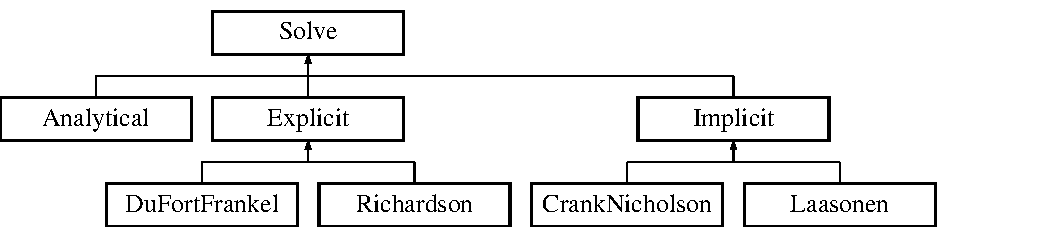
\includegraphics[height=3.000000cm]{class_solve}
\end{center}
\end{figure}
\subsection*{Public Member Functions}
\begin{DoxyCompactItemize}
\item 
\hyperlink{class_solve_ac437f1307c9d4669205ac7d370a55ffc}{Solve} ()
\item 
\hyperlink{class_solve_a1e0efad6dcf6b09759dd38df7aa08db8}{Solve} (double \hyperlink{class_solve_ab6b73352e9bca73bad1b133fc84f008c}{D}, double \hyperlink{class_solve_a324c747af91a26a206d7772853b8655e}{Tin}, double \hyperlink{class_solve_a7145536b49fb1ac4d2f36f800d118616}{Tsun}, double \hyperlink{class_solve_ac1befb9c006f895fb0517e19c412ca57}{dt}, double \hyperlink{class_solve_a21b9b8118f508e079f066d2ce2816dd1}{dx})
\item 
virtual void \hyperlink{class_solve_a1a56722993fdabea9928637d7dd8a2c7}{solve} (double t)
\item 
double \hyperlink{class_solve_a0edcf69bae8414576fbb1b35ba395a1c}{getD} ()
\item 
void \hyperlink{class_solve_ab313553673e1e419bcc150be13d3d58b}{setD} (double \hyperlink{class_solve_ab6b73352e9bca73bad1b133fc84f008c}{D})
\item 
double \hyperlink{class_solve_a7d9d481ed1bf8bbfc5bf37517e2a12c6}{get\+Tin} ()
\item 
void \hyperlink{class_solve_acef277ebf827a664b4378285a1fbeca3}{set\+Tin} (double \hyperlink{class_solve_a324c747af91a26a206d7772853b8655e}{Tin})
\item 
double \hyperlink{class_solve_afad3694fc830b80135a316eea2c0c279}{get\+Tsun} ()
\item 
void \hyperlink{class_solve_a2088840c7117930845bc61444cbba285}{set\+Tsun} (double \hyperlink{class_solve_a7145536b49fb1ac4d2f36f800d118616}{Tsun})
\item 
double \hyperlink{class_solve_a981e11c3c390bc54041a8e60ebdcc4bf}{getdt} ()
\item 
void \hyperlink{class_solve_af05556226469b3b7d4773b61342fbf73}{setdt} (double \hyperlink{class_solve_ac1befb9c006f895fb0517e19c412ca57}{dt})
\item 
double \hyperlink{class_solve_aad066a37070623f3c1bfb5f001fd2a50}{getdx} ()
\item 
void \hyperlink{class_solve_a60a27ba683584477189dc9c260c75127}{setdx} (double \hyperlink{class_solve_a21b9b8118f508e079f066d2ce2816dd1}{dx})
\end{DoxyCompactItemize}
\subsection*{Public Attributes}
\begin{DoxyCompactItemize}
\item 
double \hyperlink{class_solve_ab6b73352e9bca73bad1b133fc84f008c}{D}
\item 
double \hyperlink{class_solve_a324c747af91a26a206d7772853b8655e}{Tin}
\item 
double \hyperlink{class_solve_a7145536b49fb1ac4d2f36f800d118616}{Tsun}
\item 
double \hyperlink{class_solve_ac1befb9c006f895fb0517e19c412ca57}{dt}
\item 
double \hyperlink{class_solve_a21b9b8118f508e079f066d2ce2816dd1}{dx}
\item 
double \hyperlink{class_solve_a8007aa7266c3ba3207ce233d54d720d7}{r}
\item 
int \hyperlink{class_solve_acc2a34441a699bf1e68f730a1bbe7774}{n}
\item 
int \hyperlink{class_solve_a95de020d455d886e667b8307d7efed55}{L}
\end{DoxyCompactItemize}


\subsection{Detailed Description}
It\textquotesingle{}s the main base classes of the program ~\newline
 It implements the data needed to solve the problem with each method ~\newline
 In those date we can find\+: ~\newline
-\/D the diffusity in ft$^\wedge$2/hr ~\newline
-\/\+Tin The initial temperature ~\newline
-\/\+Tsun The temperature of of the two surfaces of the wall at x0 and xn ~\newline
-\/dt The gap in time between n and n+1 ~\newline
-\/dx The gap in space between i and i+1

The \hyperlink{class_solve}{Solve} class provides\+: ~\newline
-\/basic constructor that will be reused in all derivated class ~\newline
-\/set and get function for each variable set by the user ~\newline
-\/a virtual function \hyperlink{class_solve_a1a56722993fdabea9928637d7dd8a2c7}{solve()} that will be use in the derived function to solve the problem 

\subsection{Constructor \& Destructor Documentation}
\mbox{\Hypertarget{class_solve_ac437f1307c9d4669205ac7d370a55ffc}\label{class_solve_ac437f1307c9d4669205ac7d370a55ffc}} 
\index{Solve@{Solve}!Solve@{Solve}}
\index{Solve@{Solve}!Solve@{Solve}}
\subsubsection{\texorpdfstring{Solve()}{Solve()}\hspace{0.1cm}{\footnotesize\ttfamily [1/2]}}
{\footnotesize\ttfamily Solve\+::\+Solve (\begin{DoxyParamCaption}{ }\end{DoxyParamCaption})}

Default constructor. Initialize a \hyperlink{class_solve}{Solve} element with the needed element set to 1 \begin{DoxySeeAlso}{See also}
\hyperlink{class_solve_a1e0efad6dcf6b09759dd38df7aa08db8}{Solve(double D, double Tin, double Tsun, double dt, double dx)}
\end{DoxySeeAlso}
Default constructor -\/ Set all the value to 1 \mbox{\Hypertarget{class_solve_a1e0efad6dcf6b09759dd38df7aa08db8}\label{class_solve_a1e0efad6dcf6b09759dd38df7aa08db8}} 
\index{Solve@{Solve}!Solve@{Solve}}
\index{Solve@{Solve}!Solve@{Solve}}
\subsubsection{\texorpdfstring{Solve()}{Solve()}\hspace{0.1cm}{\footnotesize\ttfamily [2/2]}}
{\footnotesize\ttfamily Solve\+::\+Solve (\begin{DoxyParamCaption}\item[{double}]{D,  }\item[{double}]{Tin,  }\item[{double}]{Tsun,  }\item[{double}]{dt,  }\item[{double}]{dx }\end{DoxyParamCaption})}

Initialize a \hyperlink{class_solve}{Solve} element with the needed element to solve the problem

Default constructor -\/  the value of D, Tin, Tsun, dt, dx and L and create r and n which are to simplified calculation in the derived classes. 

\subsection{Member Function Documentation}
\mbox{\Hypertarget{class_solve_a0edcf69bae8414576fbb1b35ba395a1c}\label{class_solve_a0edcf69bae8414576fbb1b35ba395a1c}} 
\index{Solve@{Solve}!getD@{getD}}
\index{getD@{getD}!Solve@{Solve}}
\subsubsection{\texorpdfstring{get\+D()}{getD()}}
{\footnotesize\ttfamily double Solve\+::getD (\begin{DoxyParamCaption}{ }\end{DoxyParamCaption})}

Normal get method that returns double, the number D \begin{DoxyReturn}{Returns}
double. The value of D 
\end{DoxyReturn}
\mbox{\Hypertarget{class_solve_a981e11c3c390bc54041a8e60ebdcc4bf}\label{class_solve_a981e11c3c390bc54041a8e60ebdcc4bf}} 
\index{Solve@{Solve}!getdt@{getdt}}
\index{getdt@{getdt}!Solve@{Solve}}
\subsubsection{\texorpdfstring{getdt()}{getdt()}}
{\footnotesize\ttfamily double Solve\+::getdt (\begin{DoxyParamCaption}{ }\end{DoxyParamCaption})}

Normal get method that returns double, the number dt \begin{DoxyReturn}{Returns}
double. The value of dt 
\end{DoxyReturn}
\mbox{\Hypertarget{class_solve_aad066a37070623f3c1bfb5f001fd2a50}\label{class_solve_aad066a37070623f3c1bfb5f001fd2a50}} 
\index{Solve@{Solve}!getdx@{getdx}}
\index{getdx@{getdx}!Solve@{Solve}}
\subsubsection{\texorpdfstring{getdx()}{getdx()}}
{\footnotesize\ttfamily double Solve\+::getdx (\begin{DoxyParamCaption}{ }\end{DoxyParamCaption})}

Normal get method that returns double, the number dt \begin{DoxyReturn}{Returns}
double. The value of dx 
\end{DoxyReturn}
\mbox{\Hypertarget{class_solve_a7d9d481ed1bf8bbfc5bf37517e2a12c6}\label{class_solve_a7d9d481ed1bf8bbfc5bf37517e2a12c6}} 
\index{Solve@{Solve}!get\+Tin@{get\+Tin}}
\index{get\+Tin@{get\+Tin}!Solve@{Solve}}
\subsubsection{\texorpdfstring{get\+Tin()}{getTin()}}
{\footnotesize\ttfamily double Solve\+::get\+Tin (\begin{DoxyParamCaption}{ }\end{DoxyParamCaption})}

Normal get method that returns double, the number Tin \begin{DoxyReturn}{Returns}
double. The value of Tin 
\end{DoxyReturn}
\mbox{\Hypertarget{class_solve_afad3694fc830b80135a316eea2c0c279}\label{class_solve_afad3694fc830b80135a316eea2c0c279}} 
\index{Solve@{Solve}!get\+Tsun@{get\+Tsun}}
\index{get\+Tsun@{get\+Tsun}!Solve@{Solve}}
\subsubsection{\texorpdfstring{get\+Tsun()}{getTsun()}}
{\footnotesize\ttfamily double Solve\+::get\+Tsun (\begin{DoxyParamCaption}{ }\end{DoxyParamCaption})}

Normal get method that returns double, the number Tsun \begin{DoxyReturn}{Returns}
double. The value of Tsun 
\end{DoxyReturn}
\mbox{\Hypertarget{class_solve_ab313553673e1e419bcc150be13d3d58b}\label{class_solve_ab313553673e1e419bcc150be13d3d58b}} 
\index{Solve@{Solve}!setD@{setD}}
\index{setD@{setD}!Solve@{Solve}}
\subsubsection{\texorpdfstring{set\+D()}{setD()}}
{\footnotesize\ttfamily void Solve\+::setD (\begin{DoxyParamCaption}\item[{double}]{D }\end{DoxyParamCaption})}

\mbox{\Hypertarget{class_solve_af05556226469b3b7d4773b61342fbf73}\label{class_solve_af05556226469b3b7d4773b61342fbf73}} 
\index{Solve@{Solve}!setdt@{setdt}}
\index{setdt@{setdt}!Solve@{Solve}}
\subsubsection{\texorpdfstring{setdt()}{setdt()}}
{\footnotesize\ttfamily void Solve\+::setdt (\begin{DoxyParamCaption}\item[{double}]{dt }\end{DoxyParamCaption})}

Normal set method that set the value of the number dt \mbox{\Hypertarget{class_solve_a60a27ba683584477189dc9c260c75127}\label{class_solve_a60a27ba683584477189dc9c260c75127}} 
\index{Solve@{Solve}!setdx@{setdx}}
\index{setdx@{setdx}!Solve@{Solve}}
\subsubsection{\texorpdfstring{setdx()}{setdx()}}
{\footnotesize\ttfamily void Solve\+::setdx (\begin{DoxyParamCaption}\item[{double}]{dx }\end{DoxyParamCaption})}

Normal set method that set the value of the number dx \mbox{\Hypertarget{class_solve_acef277ebf827a664b4378285a1fbeca3}\label{class_solve_acef277ebf827a664b4378285a1fbeca3}} 
\index{Solve@{Solve}!set\+Tin@{set\+Tin}}
\index{set\+Tin@{set\+Tin}!Solve@{Solve}}
\subsubsection{\texorpdfstring{set\+Tin()}{setTin()}}
{\footnotesize\ttfamily void Solve\+::set\+Tin (\begin{DoxyParamCaption}\item[{double}]{Tin }\end{DoxyParamCaption})}

Normal set method that set the value of the number Tsun \mbox{\Hypertarget{class_solve_a2088840c7117930845bc61444cbba285}\label{class_solve_a2088840c7117930845bc61444cbba285}} 
\index{Solve@{Solve}!set\+Tsun@{set\+Tsun}}
\index{set\+Tsun@{set\+Tsun}!Solve@{Solve}}
\subsubsection{\texorpdfstring{set\+Tsun()}{setTsun()}}
{\footnotesize\ttfamily void Solve\+::set\+Tsun (\begin{DoxyParamCaption}\item[{double}]{Tsun }\end{DoxyParamCaption})}

Normal set method that set the value of the number Tin \mbox{\Hypertarget{class_solve_a1a56722993fdabea9928637d7dd8a2c7}\label{class_solve_a1a56722993fdabea9928637d7dd8a2c7}} 
\index{Solve@{Solve}!solve@{solve}}
\index{solve@{solve}!Solve@{Solve}}
\subsubsection{\texorpdfstring{solve()}{solve()}}
{\footnotesize\ttfamily void Solve\+::solve (\begin{DoxyParamCaption}\item[{double}]{t }\end{DoxyParamCaption})\hspace{0.3cm}{\ttfamily [virtual]}}

Virtual methods that solve the problem for each scheme depending in which class the objet is define and print it in the consol.  the solve class it doesn\textquotesingle{}t do anything

Virtual method -\/ Not defined here 

Reimplemented in \hyperlink{class_implicit_a027adb4276376991f75fcffbd34740b3}{Implicit}, \hyperlink{class_explicit_ac99aa17bfd95f66b33e5c0ecf0e53785}{Explicit}, \hyperlink{class_analytical_a8fe1d5769bb516115a31719222eb9ae5}{Analytical}, \hyperlink{class_laasonen_aaa49ab7d15fbfef94a57a0e89977d1c6}{Laasonen}, \hyperlink{class_du_fort_frankel_a73204223c7ace1e3f95e5d89d02c5208}{Du\+Fort\+Frankel}, \hyperlink{class_richardson_ab8dd2ff0e58c11092fead4d45a4f5c64}{Richardson}, and \hyperlink{class_crank_nicholson_a999d04c6ef97b0794f66584f9192dbee}{Crank\+Nicholson}.



\subsection{Member Data Documentation}
\mbox{\Hypertarget{class_solve_ab6b73352e9bca73bad1b133fc84f008c}\label{class_solve_ab6b73352e9bca73bad1b133fc84f008c}} 
\index{Solve@{Solve}!D@{D}}
\index{D@{D}!Solve@{Solve}}
\subsubsection{\texorpdfstring{D}{D}}
{\footnotesize\ttfamily double Solve\+::D}

\mbox{\Hypertarget{class_solve_ac1befb9c006f895fb0517e19c412ca57}\label{class_solve_ac1befb9c006f895fb0517e19c412ca57}} 
\index{Solve@{Solve}!dt@{dt}}
\index{dt@{dt}!Solve@{Solve}}
\subsubsection{\texorpdfstring{dt}{dt}}
{\footnotesize\ttfamily double Solve\+::dt}

\mbox{\Hypertarget{class_solve_a21b9b8118f508e079f066d2ce2816dd1}\label{class_solve_a21b9b8118f508e079f066d2ce2816dd1}} 
\index{Solve@{Solve}!dx@{dx}}
\index{dx@{dx}!Solve@{Solve}}
\subsubsection{\texorpdfstring{dx}{dx}}
{\footnotesize\ttfamily double Solve\+::dx}

\mbox{\Hypertarget{class_solve_a95de020d455d886e667b8307d7efed55}\label{class_solve_a95de020d455d886e667b8307d7efed55}} 
\index{Solve@{Solve}!L@{L}}
\index{L@{L}!Solve@{Solve}}
\subsubsection{\texorpdfstring{L}{L}}
{\footnotesize\ttfamily int Solve\+::L}

\mbox{\Hypertarget{class_solve_acc2a34441a699bf1e68f730a1bbe7774}\label{class_solve_acc2a34441a699bf1e68f730a1bbe7774}} 
\index{Solve@{Solve}!n@{n}}
\index{n@{n}!Solve@{Solve}}
\subsubsection{\texorpdfstring{n}{n}}
{\footnotesize\ttfamily int Solve\+::n}

\mbox{\Hypertarget{class_solve_a8007aa7266c3ba3207ce233d54d720d7}\label{class_solve_a8007aa7266c3ba3207ce233d54d720d7}} 
\index{Solve@{Solve}!r@{r}}
\index{r@{r}!Solve@{Solve}}
\subsubsection{\texorpdfstring{r}{r}}
{\footnotesize\ttfamily double Solve\+::r}

\mbox{\Hypertarget{class_solve_a324c747af91a26a206d7772853b8655e}\label{class_solve_a324c747af91a26a206d7772853b8655e}} 
\index{Solve@{Solve}!Tin@{Tin}}
\index{Tin@{Tin}!Solve@{Solve}}
\subsubsection{\texorpdfstring{Tin}{Tin}}
{\footnotesize\ttfamily double Solve\+::\+Tin}

\mbox{\Hypertarget{class_solve_a7145536b49fb1ac4d2f36f800d118616}\label{class_solve_a7145536b49fb1ac4d2f36f800d118616}} 
\index{Solve@{Solve}!Tsun@{Tsun}}
\index{Tsun@{Tsun}!Solve@{Solve}}
\subsubsection{\texorpdfstring{Tsun}{Tsun}}
{\footnotesize\ttfamily double Solve\+::\+Tsun}



The documentation for this class was generated from the following files\+:\begin{DoxyCompactItemize}
\item 
Solver/\hyperlink{solve_8h}{solve.\+h}\item 
Solver/\hyperlink{solve_8cpp}{solve.\+cpp}\end{DoxyCompactItemize}

\hypertarget{class_vector}{}\section{Vector Class Reference}
\label{class_vector}\index{Vector@{Vector}}


{\ttfamily \#include $<$vector.\+h$>$}

Inheritance diagram for Vector\+:\begin{figure}[H]
\begin{center}
\leavevmode
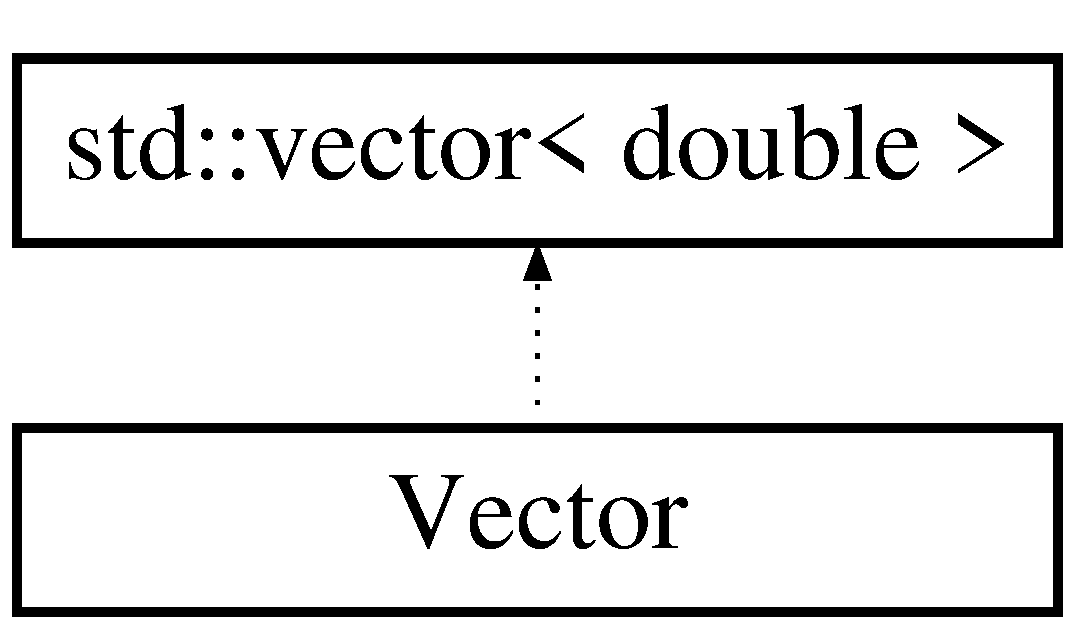
\includegraphics[height=2.000000cm]{class_vector}
\end{center}
\end{figure}
\subsection*{Public Member Functions}
\begin{DoxyCompactItemize}
\item 
\hyperlink{class_vector_a6f80c73b5f18dcf3f8e36065bdc8b9e5}{Vector} ()
\item 
\hyperlink{class_vector_acbdf66550f2caa0a64e0b356fb63a277}{Vector} (int Num)
\item 
\hyperlink{class_vector_a5f04e343b7306ad11f8a82c89b486764}{Vector} (const \hyperlink{class_vector}{Vector} \&v)
\item 
\hyperlink{class_vector}{Vector} \& \hyperlink{class_vector_ae48c467a9f65d60e2f7455aba4ca1239}{operator=} (const \hyperlink{class_vector}{Vector} \&v)
\item 
bool \hyperlink{class_vector_ade5fbd0cd01b034d1907e0c93433320c}{operator==} (const \hyperlink{class_vector}{Vector} \&v) const
\item 
int \hyperlink{class_vector_afbb7966ec4107c43ec15cccc47fcaef7}{get\+Size} () const
\item 
double \hyperlink{class_vector_a6752a90058ddef427ca6aed12946a737}{one\+\_\+norm} () const
\item 
double \hyperlink{class_vector_a4f501290a50d057bb6c57ea64d7e70a4}{two\+\_\+norm} () const
\item 
double \hyperlink{class_vector_a50b72131eaf3698a9876d99ab6912a32}{uniform\+\_\+norm} () const
\end{DoxyCompactItemize}


\subsection{Detailed Description}
A vector class for data storage of a 1D array of doubles ~\newline
 The implementation is derived from the standard container vector std\+::vector ~\newline
 We use private inheritance to base our vector upon the library version whilst  us to expose only those base class functions we wish to use -\/ in this  the array access operator \mbox{[}\mbox{]}

The \hyperlink{class_vector}{Vector} class provides\+: ~\newline
-\/basic constructors for creating vector obcjet from other vector object, or by creating empty vector of a given size, ~\newline
-\/input and oput operation via $>$$>$ and $<$$<$ operators using keyboard or file ~\newline
-\/basic operations like access via \mbox{[}\mbox{]} operator, assignment and comparision 

\subsection{Constructor \& Destructor Documentation}
\mbox{\Hypertarget{class_vector_a6f80c73b5f18dcf3f8e36065bdc8b9e5}\label{class_vector_a6f80c73b5f18dcf3f8e36065bdc8b9e5}} 
\index{Vector@{Vector}!Vector@{Vector}}
\index{Vector@{Vector}!Vector@{Vector}}
\subsubsection{\texorpdfstring{Vector()}{Vector()}\hspace{0.1cm}{\footnotesize\ttfamily [1/3]}}
{\footnotesize\ttfamily Vector\+::\+Vector (\begin{DoxyParamCaption}{ }\end{DoxyParamCaption})}

Default constructor. Intialize an empty \hyperlink{class_vector}{Vector} object \begin{DoxySeeAlso}{See also}
\hyperlink{class_vector_acbdf66550f2caa0a64e0b356fb63a277}{Vector(int Num)} 

\hyperlink{class_vector_a5f04e343b7306ad11f8a82c89b486764}{Vector(const Vector\& v)} 
\end{DoxySeeAlso}
\mbox{\Hypertarget{class_vector_acbdf66550f2caa0a64e0b356fb63a277}\label{class_vector_acbdf66550f2caa0a64e0b356fb63a277}} 
\index{Vector@{Vector}!Vector@{Vector}}
\index{Vector@{Vector}!Vector@{Vector}}
\subsubsection{\texorpdfstring{Vector()}{Vector()}\hspace{0.1cm}{\footnotesize\ttfamily [2/3]}}
{\footnotesize\ttfamily Vector\+::\+Vector (\begin{DoxyParamCaption}\item[{int}]{Num }\end{DoxyParamCaption})\hspace{0.3cm}{\ttfamily [explicit]}}

\hyperlink{class_explicit}{Explicit} alterative constructor takes an intiger. it is explicit since implicit type conversion int -\/$>$ vector doesn\textquotesingle{}t make sense Intialize \hyperlink{class_vector}{Vector} object of size Num \begin{DoxySeeAlso}{See also}
\hyperlink{class_vector_a6f80c73b5f18dcf3f8e36065bdc8b9e5}{Vector()} 

\hyperlink{class_vector_a5f04e343b7306ad11f8a82c89b486764}{Vector(const Vector\& v)} 
\end{DoxySeeAlso}

\begin{DoxyExceptions}{Exceptions}
{\em invalid\+\_\+argument} & (\char`\"{}vector size negative\char`\"{}) \\
\hline
\end{DoxyExceptions}

\begin{DoxyParams}{Parameters}
{\em Num} & int. Size of a vector \\
\hline
\end{DoxyParams}
\mbox{\Hypertarget{class_vector_a5f04e343b7306ad11f8a82c89b486764}\label{class_vector_a5f04e343b7306ad11f8a82c89b486764}} 
\index{Vector@{Vector}!Vector@{Vector}}
\index{Vector@{Vector}!Vector@{Vector}}
\subsubsection{\texorpdfstring{Vector()}{Vector()}\hspace{0.1cm}{\footnotesize\ttfamily [3/3]}}
{\footnotesize\ttfamily Vector\+::\+Vector (\begin{DoxyParamCaption}\item[{const \hyperlink{class_vector}{Vector} \&}]{v }\end{DoxyParamCaption})}

Copy constructor takes an \hyperlink{class_vector}{Vector} object reference. Intialize \hyperlink{class_vector}{Vector} object with another \hyperlink{class_vector}{Vector} object \begin{DoxySeeAlso}{See also}
\hyperlink{class_vector_a6f80c73b5f18dcf3f8e36065bdc8b9e5}{Vector()} 

\hyperlink{class_vector_acbdf66550f2caa0a64e0b356fb63a277}{Vector(int Num)} 
\end{DoxySeeAlso}


\subsection{Member Function Documentation}
\mbox{\Hypertarget{class_vector_afbb7966ec4107c43ec15cccc47fcaef7}\label{class_vector_afbb7966ec4107c43ec15cccc47fcaef7}} 
\index{Vector@{Vector}!get\+Size@{get\+Size}}
\index{get\+Size@{get\+Size}!Vector@{Vector}}
\subsubsection{\texorpdfstring{get\+Size()}{getSize()}}
{\footnotesize\ttfamily int Vector\+::get\+Size (\begin{DoxyParamCaption}{ }\end{DoxyParamCaption}) const}

Normal get method that returns integer, the size of the vector \begin{DoxyReturn}{Returns}
int. the size of the vector 
\end{DoxyReturn}
\mbox{\Hypertarget{class_vector_a6752a90058ddef427ca6aed12946a737}\label{class_vector_a6752a90058ddef427ca6aed12946a737}} 
\index{Vector@{Vector}!one\+\_\+norm@{one\+\_\+norm}}
\index{one\+\_\+norm@{one\+\_\+norm}!Vector@{Vector}}
\subsubsection{\texorpdfstring{one\+\_\+norm()}{one\_norm()}}
{\footnotesize\ttfamily double Vector\+::one\+\_\+norm (\begin{DoxyParamCaption}{ }\end{DoxyParamCaption}) const}

Normal public method that returns a double. It returns L1 norm of vector \begin{DoxySeeAlso}{See also}
\hyperlink{class_vector_a4f501290a50d057bb6c57ea64d7e70a4}{two\+\_\+norm()const} 

\hyperlink{class_vector_a50b72131eaf3698a9876d99ab6912a32}{uniform\+\_\+norm()const} 
\end{DoxySeeAlso}
\begin{DoxyReturn}{Returns}
double. vectors L1 norm 
\end{DoxyReturn}
\mbox{\Hypertarget{class_vector_ae48c467a9f65d60e2f7455aba4ca1239}\label{class_vector_ae48c467a9f65d60e2f7455aba4ca1239}} 
\index{Vector@{Vector}!operator=@{operator=}}
\index{operator=@{operator=}!Vector@{Vector}}
\subsubsection{\texorpdfstring{operator=()}{operator=()}}
{\footnotesize\ttfamily \hyperlink{class_vector}{Vector} \& Vector\+::operator= (\begin{DoxyParamCaption}\item[{const \hyperlink{class_vector}{Vector} \&}]{v }\end{DoxyParamCaption})}

Overloaded assignment operator \begin{DoxySeeAlso}{See also}
\hyperlink{class_vector_ade5fbd0cd01b034d1907e0c93433320c}{operator==(const Vector\& v)const} 
\end{DoxySeeAlso}

\begin{DoxyParams}{Parameters}
{\em v} & \hyperlink{class_vector}{Vector} to assign from \\
\hline
\end{DoxyParams}
\begin{DoxyReturn}{Returns}
the object on the left of the assignment 
\end{DoxyReturn}

\begin{DoxyParams}{Parameters}
{\em v} & Vecto\&. \hyperlink{class_vector}{Vector} to assign from \\
\hline
\end{DoxyParams}
\mbox{\Hypertarget{class_vector_ade5fbd0cd01b034d1907e0c93433320c}\label{class_vector_ade5fbd0cd01b034d1907e0c93433320c}} 
\index{Vector@{Vector}!operator==@{operator==}}
\index{operator==@{operator==}!Vector@{Vector}}
\subsubsection{\texorpdfstring{operator==()}{operator==()}}
{\footnotesize\ttfamily bool Vector\+::operator== (\begin{DoxyParamCaption}\item[{const \hyperlink{class_vector}{Vector} \&}]{v }\end{DoxyParamCaption}) const}

Overloaded comparison operator returns true if vectors are the same within a tolerance (1.\+e-\/07) \begin{DoxySeeAlso}{See also}
\hyperlink{class_vector_ae48c467a9f65d60e2f7455aba4ca1239}{operator=(const Vector\& v)} 

operator\mbox{[}$\,$\mbox{]}(int i) 

operator\mbox{[}$\,$\mbox{]}(int i)const 
\end{DoxySeeAlso}
\begin{DoxyReturn}{Returns}
bool. true or false 
\end{DoxyReturn}

\begin{DoxyExceptions}{Exceptions}
{\em invalid\+\_\+argument} & (\char`\"{}incompatible vector sizes\textbackslash{}n\char`\"{}) \\
\hline
\end{DoxyExceptions}

\begin{DoxyParams}{Parameters}
{\em v} & \hyperlink{class_vector}{Vector}\&. vector to compare \\
\hline
\end{DoxyParams}
\mbox{\Hypertarget{class_vector_a4f501290a50d057bb6c57ea64d7e70a4}\label{class_vector_a4f501290a50d057bb6c57ea64d7e70a4}} 
\index{Vector@{Vector}!two\+\_\+norm@{two\+\_\+norm}}
\index{two\+\_\+norm@{two\+\_\+norm}!Vector@{Vector}}
\subsubsection{\texorpdfstring{two\+\_\+norm()}{two\_norm()}}
{\footnotesize\ttfamily double Vector\+::two\+\_\+norm (\begin{DoxyParamCaption}{ }\end{DoxyParamCaption}) const}

Normal public method that returns a double. It returns L2 norm of vector \begin{DoxySeeAlso}{See also}
\hyperlink{class_vector_a6752a90058ddef427ca6aed12946a737}{one\+\_\+norm()const} 

\hyperlink{class_vector_a50b72131eaf3698a9876d99ab6912a32}{uniform\+\_\+norm()const} 
\end{DoxySeeAlso}
\begin{DoxyReturn}{Returns}
double. vectors L2 norm 
\end{DoxyReturn}
\mbox{\Hypertarget{class_vector_a50b72131eaf3698a9876d99ab6912a32}\label{class_vector_a50b72131eaf3698a9876d99ab6912a32}} 
\index{Vector@{Vector}!uniform\+\_\+norm@{uniform\+\_\+norm}}
\index{uniform\+\_\+norm@{uniform\+\_\+norm}!Vector@{Vector}}
\subsubsection{\texorpdfstring{uniform\+\_\+norm()}{uniform\_norm()}}
{\footnotesize\ttfamily double Vector\+::uniform\+\_\+norm (\begin{DoxyParamCaption}{ }\end{DoxyParamCaption}) const}

Normal public method that returns a double. It returns L\+\_\+max norm of vector \begin{DoxySeeAlso}{See also}
\hyperlink{class_vector_a6752a90058ddef427ca6aed12946a737}{one\+\_\+norm()const} 

\hyperlink{class_vector_a4f501290a50d057bb6c57ea64d7e70a4}{two\+\_\+norm()const} 
\end{DoxySeeAlso}

\begin{DoxyExceptions}{Exceptions}
{\em out\+\_\+of\+\_\+range} & (\char`\"{}vector access error\char`\"{}) vector has zero size \\
\hline
\end{DoxyExceptions}
\begin{DoxyReturn}{Returns}
double. vectors Lmax norm 
\end{DoxyReturn}


The documentation for this class was generated from the following files\+:\begin{DoxyCompactItemize}
\item 
Class/\+Use\+Class/vector.\+h\item 
Class/\+Use\+Class/vector.\+cpp\end{DoxyCompactItemize}

%--- End generated contents ---

% Index
\backmatter
\newpage
\phantomsection
\clearemptydoublepage
\addcontentsline{toc}{chapter}{Index}
\printindex

\end{document}
